\documentclass[11pt]{article}

\usepackage[margin=1in]{geometry}
\usepackage{amsmath,amssymb,amsthm}
\usepackage{graphicx}
\usepackage[T1]{fontenc}
\usepackage{helvet}
\renewcommand{\familydefault}{\sfdefault}
\usepackage{xcolor}
\usepackage{natbib}
\usepackage{hyperref}
\usepackage{setspace}
\usepackage{lineno}
\renewcommand\linenumberfont{\normalfont\footnotesize\ttfamily\color{gray}}

% Dark mode: activated via \def\darkmode{} on the command line
\ifdefined\darkmode
  \pagecolor{black}
  \color{white}
  \hypersetup{colorlinks=true, linkcolor=cyan, citecolor=cyan, urlcolor=cyan}
\fi

% Uniform font size for title and sections
\usepackage{titlesec}
\titleformat{\section}{\normalsize\bfseries}{\thesection}{1em}{}
\titleformat{\subsection}{\normalsize\bfseries\itshape}{\thesubsection}{1em}{}
\titleformat{\subsubsection}{\normalsize\itshape}{\thesubsubsection}{1em}{}

\onehalfspacing
\linenumbers

\begin{document}

\noindent\textbf{The impact of punctuated infectiousness on infectious disease dynamics}
\vskip 1.5em

\begin{abstract}
\noindent\small
\end{abstract}
\vskip 1.5em

\clearpage 
\section{Introduction}

The trajectory of an epidemic depends on two fundamental quantities: the basic reproduction number ($R_0$), which is the expected number of secondary infections that an infectious person will produce in an otherwise susceptible population; and the generation interval distribution ($g(\tau)$), which is the distribution of times at which those secondary infections are expected to occur relative to the index case's infection time ($\tau = 0$) \citep{wallinga_how_2007}. These quantities can be combined into a single object, the ``infectiousness profile'', defined as $A(\tau) = R_0 g(\tau)$, which describes a person's expected contribution to transmission and how it is distributed over time \citep{breda_formulation_2012}. 

The reproduction number and the generation interval distribution are both expectations taken over a large population. At the individual level, the individual reproduction number, $\nu_i$, is the expected number of infections that a particular person $i$ will produce, such that $R_0 = E_i[\nu_i]$ \citep{lloyd-smith_superspreading_2005}. Similarly, the ``individual infectiousness profile'' or ``infectiousness kernel'', $a_i(\tau)$, describes how a particular person's infectiousness is distributed over time, with $A(\tau) = E_i[a_i(\tau)]$ \citep{champredon_intrinsic_2015, svensson_note_2007}. 

Estimating $R_0$ and $g(\tau)$ (and thus $A(\tau)$) is critical for modeling epidemic dynamics and designing interventions. However, the shape of the individual infectiousness profile $a_i(\tau)$ is poorly understood for many pathogens. There are two main reasons for this: we lack a clear understanding of whether, and how, the shape of $a_i(\tau)$ impacts epidemic dynamics beyond what $A(\tau)$ can provide, and thus lack motivation to target $a_i(\tau)$ in study designs; and we lack study designs and inferential methods capable of inferring $a_i(\tau)$ independently of $A(\tau)$. 

Often, a modeling choice is made to assume $a_i(\tau) \equiv A(\tau)$. However, it is likely that the full variability in $A(\tau)$ is made up of both within-individual and between-individual variation, implying $a_i(\tau)$ is generally narrower than $A(\tau)$. Emphasizing this point, some evidence suggests that the period when SARS-CoV-2 and influenza can transmit explosively is short, lasting less than a day \citep{goyal_viral_2021}, sugesting that $a_i(\tau)$ may in some cases be much narrower than $A(\tau)$, with much of the variation in $A(\tau)$ arising from variation between individuals and on when their peak infectiousness occurs. These considerations are sometimes built into disease transmission models, but we lack a comprehensive understanding of how the punctuatedness of $a_i(\tau)$, independent of other factors, impacts disease transmission dynamics, and we lack a clear framework for incorporating $a_i(\tau)$ into the foundational disease transmission modeling frameworks upon which virtually all others are based. 

At the individual level, communicating about the likely timing of a person's infectiousness is important: it is good to know if you will be very infectious for a short time, or mildly infectious for a long time, so that you can shape your behavior accordingly. Additionally, a punctuated individual infectiousness kernel could impact epidemic dynamics. Even if the epidemic has the same mean-field behavior, it could impact the stochastic dynamics via highly synchronized transmission events, especially when an outbreak is small. It could interplay with control measures, especially those designed to intervene on infectiousness at the individual level like test- or symptom-based screening and isolation. Indeed, the impact of the punctuatedness of the individual infectiousness kernel has been examined as a sensitivity analysis in various epidemiological studies \citep{larremore_test_2021} {\bf Others?}. Stochastic effects are known to cascade through macroscopic features of an epidemic \citep{morris_computation_2024}. However, we lack a comprehensive understanding of how the sharpness of the individual infectiousness kernel, independent of other features like the individual reproduction number, basic reproduction number, and generation interval distribution, impacts epidemic dynamics under both uncontrolled and controlled settings. Furthermore, we lack an understanding of how to measure the shape of the individual infectiousness kernel reliably, along with the settings when the kernel's shape is statistically identifiable.

The main goal: holding $A(\tau)$ constant, how do different choices of $a_i(\tau)$ impact epidemic dynamics? And how would we know what $a(\tau)$ looks like? 

% ⏺ The literature search is done. Here's the key finding upfront: no paper makes your core results
%   redundant. But there are several important papers to cite and position against. Let me give you the
%    organized summary.

%   Papers you must cite and distinguish from

%   Most structurally similar:
%   - Yan (2008), J. Theor. Biol. — Decomposes the generation interval into latent + infectious periods
%    and studies how the split affects dynamics. Key difference: Yan changes A(τ) when varying the
%   split; you fix it. Also purely deterministic.
%   - Lloyd (2001a,b), Theor. Pop. Biol. & Proc. R. Soc. B — Shows narrower (Erlang) infectious periods
%    destabilize deterministic dynamics. Conceptually analogous (many E stages vs few I stages ≈
%   varying κ), but again changes A(τ), and is deterministic only.
%   - Wearing, Rohani & Keeling (2005), PLoS Medicine — Distribution shape of the infectious period
%   affects R0 estimates, peak size, intervention timing. Motivates your question but varies the
%   population-level profile.

%   Generation interval variance and growth rates:
%   - Wallinga & Lipsitch (2007), Proc. R. Soc. B — Foundational r-to-R0 mapping via GI shape. Their
%   "all GI equal to the mean" upper bound corresponds to your κ→0. Your project shows r and R0 are
%   κ-invariant by construction, but stochastic variability is not.
%   - Park, Champredon, Weitz & Dushoff (2019), Epidemics — Extends Wallinga-Lipsitch with Gamma GI
%   methods. Machinery you use, but no individual-level decomposition.

%   The W/time-shift framework:
%   - Morris, Maclean & Black (2024), J. Math. Biol. — Already cited. Provides the time-shift framework
%    but does not study how W depends on individual-level kernel decomposition or anything like κ.
%   - Jagers (1975), Nerman (1981), Jagers & Nerman (1984) — Foundational CMJ theory for W. Your Var(W)
%    as a function of κ extends their general results.

%   Superspreading / intervention papers:
%   - Lloyd-Smith et al. (2005), Nature — Foundational for overdispersion in offspring number. Does not
%    consider temporal variation. Your result that punctuated infectiousness + periodic contacts
%   generates overdispersion without R_i heterogeneity is a genuinely new mechanism.
%   - Goyal et al. (2021), eLife — Closest to your overdispersion mechanism (concentrated viral load +
%   heterogeneous contacts), but simulation-only, no analytical decomposition, no closed-form k(κ).
%   - Fraser, Riley, Anderson & Ferguson (2004), PNAS — Controllability depends on pre-symptomatic
%   transmission fraction θ. Your F_κ(δ_sym) generalises their θ by showing it depends on κ. They treat
%    it as a fixed pathogen property.
%   - Champredon & Dushoff (2015), Proc. R. Soc. B — Intrinsic vs realized generation intervals, but
%   focused on how dynamics filter the distribution, not on different individual kernels producing the
%   same population kernel.

%   What's genuinely novel in your project

%   1. The κ-parameterised family — a one-parameter family of individual infectiousness profiles that
%   all share the same population-level A(τ) via Gamma additivity. Nobody has formalised this
%   non-identifiability.
%   2. Var(W) as a function of κ — closed-form dependence of stochastic epidemic variability on the
%   individual-level decomposition, holding A(τ) and R0 fixed.
%   3. "Temporal superspreading" — punctuated infectiousness interacting with periodic contacts to
%   generate overdispersed offspring counts. The closed-form k(κ) is new.
%   4. Intervention effectiveness varying with κ — no paper examines how κ affects isolation/contact
%   tracing while holding A(τ) fixed.

%   Recommended follow-up searches

%   The agent couldn't access Google Scholar directly, so I'd suggest checking for 2025–2026 papers by
%   Morris's group, Park & Dushoff, Britton/Ball/Trapman, and Kucharski using terms like "clustered
%   transmission events," "correlated infection times branching process," "burstiness transmission,"
%   and "generation interval decomposition within between individual."

 \clearpage
% ////////////////////////////////////////////////////////////////////////////////////////////
\section{Modeling individual infectiousness}

\subsection{The time-shifted Gamma model}

While our interest is in the general question of how $a_i(\tau)$, independent of $A(\tau)$, impacts epidemic dynamics, we introduce here a specific modeling framework that allows us to make precise claims while capturing the essential features of the general question. We seek a definition of $a_i(\tau)$ satisfying three requirements: (i) $A(\tau) = E_i[a_i(\tau)]$, as required by definition; (ii) $\nu_i = R_0$ for all $i$, so that there is no inherent interpersonal variation in total infectiousness; and (iii) the width of $a_i(\tau)$ is governed by a single smoothness parameter $\psi \in [0,1]$, where $\psi = 1$ yields $a_i(\tau) \equiv A(\tau)$ (the smooth case, in which each person's individual infectiousness profile matches the population average) and $\psi \to 0$ makes $a_i(\tau)$ a delta function (the spike case, in which all of a person's secondary infections occur at a single moment).

To achieve this, we first assume the intrinsic generation interval distribution $g(\tau)$ follows a $\text{Gamma}(\alpha, \beta)$ distribution with rate $\beta = \alpha/\bar{g}$, where $\bar{g}$ is the mean generation time. The Gamma distribution is a common choice for describing generation interval distributions in applied epidemiology. Next, we define each person's individual generation interval distribution as
%
\begin{equation}
    g_i(\tau) = \begin{cases}
      0 & \tau \leq l_i \\
      f_\epsilon(\tau - l_i) & \tau > l_i
    \end{cases}
    \label{eq:gamma_timeshift}
\end{equation}
%
where $l_i \sim \text{Gamma}((1 - \psi)\alpha, \beta)$ is a random latent period and $f_\epsilon$ is the $\text{Gamma}(\psi\alpha, \beta)$ density ({\bf Figure \ref{fig:psi_schematic}}). 

Setting $a_i(\tau) = R_0\,g_i(\tau)$ immediately satisfies requirement~(ii). For requirement~(iii), as $\psi \to 1$ the latent period vanishes ($l_i \to 0$) and $f_\epsilon$ approaches the full $\text{Gamma}(\alpha, \beta)$ density, so $g_i(\tau) = g(\tau)$ for all $i$; as $\psi \to 0$, $f_\epsilon$ concentrates to a point mass and $g_i(\tau)$ becomes a delta function at $\tau = l_i \sim \text{Gamma}(\alpha, \beta)$. For requirement~(i), observe that the time from infection to a secondary infection attempt is $\tau = l_i + \epsilon_i$, where $\epsilon_i \sim \text{Gamma}(\psi\alpha, \beta)$ is the draw from $f_\epsilon$. Since $l_i$ and $\epsilon_i$ are independent Gamma random variables with a common rate $\beta$, their sum follows a $\text{Gamma}((1-\psi)\alpha + \psi\alpha, \beta) = \text{Gamma}(\alpha, \beta)$ distribution by the additive property of the Gamma family. Taking expectations over individuals, $E_i[g_i(\tau)] = g(\tau)$, so $E_i[a_i(\tau)] = R_0\,g(\tau) = A(\tau)$ as required. Notably, this convergence does not require the population to share a common value of $\psi$: individual-specific values $\psi_i$ drawn from any distribution on $[0,1]$ still yield $E_i[a_i(\tau)] = A(\tau)$ ({\bf Supplementary Methods}).

\begin{figure}[ht]
\centering

\includegraphics[width=\textwidth]{figures/pdf/psi_schematic_2.pdf}
\caption{{\bf \boldmath Individual infectiousness profiles generated using the Gamma time-shift model.}  }
\label{fig:psi_schematic}
\end{figure}

% \begin{figure}[ht]
%     \centering
%     % 
\includegraphics[width=.5\textwidth]{figures/stock.png}
%     \newcommand{\panelbox}[2]{\framebox{\begin{minipage}[c][3.2cm][c]{0.3\textwidth}\centering\textbf{#1}\\\smallskip\small #2\end{minipage}}}%
%     \begin{tabular}{@{}ccc@{}}
%     \panelbox{A}{Smooth profile\\schematic} &
%     \panelbox{B}{Stepwise profile\\schematic} &
%     \panelbox{C}{Spike profile\\schematic} \\[4pt]
%     \panelbox{D}{Cumulative infections\\(smooth)} &
%     \panelbox{E}{Cumulative infections\\(stepwise)} &
%     \panelbox{F}{Cumulative infections\\(spike)} \\[4pt]
%     \panelbox{G}{Daily new infections\\(smooth)} &
%     \panelbox{H}{Daily new infections\\(stepwise)} &
%     \panelbox{I}{Daily new infections\\(spike)}
%     \end{tabular}
%     \caption{{\bf The individual infectiousness profile impacts stochastic epidemic trajectories.} (A-C) Schematic diagrams of three individual infectiousness profile families that yield equivalent SEIR-type mean-field dynamics: the smooth (A), stepwise (B), and spike (C) profiles (Eqs.~\ref{eq:a_seir_stepwise}, \ref{eq:a_seir_smooth}, \ref{eq:a_seir_spike}). (D-I) Deterministic epidemic trajectories (blue) are numerical solutions of the mean-field renewal equation model (Eq.~\ref{eq:foi}), equivalent to a standard SEIR model with latent period $1/\gamma_{\text{SEIR}} = XX$, recovery period $1/\alpha_{\text{SEIR}} = XX$, and reproduction number $R_0 = 6$. For each individual infectiousness profile family, 1,000 stochastic simulations were generated (grey), with the cumulative infections (D-F) and daily new infection counts (G-I) depicted.}
%     \label{fig:seir_sims}
% \end{figure}

%////////////////////////////////////////////////////////////////////////////////////////////

\subsection{Allowing for time-varying contacts}

The formulation above assumes time-homogeneous contacts, which is what allows $a_i(\tau)$ and $A(\tau)$ to depend only on time since infection $\tau$ and not on calendar time $t$. We follow this convention for most of our analyses. However, the interaction between punctuated infectiousness and time-varying contacts turns out to be consequential, so we briefly introduce the relevant generalization and two contact models that serve as test beds.

Under time-uniform contacts, $a_i(\tau) = \nu_i g_i(\tau)$, where $\nu_i$ and $g_i(\tau)$ are defined with respect to a reference contact process which we denote $\bar{c} \equiv 1$. To allow for time-varying contacts, we introduce a \emph{contact process} $\bm{c}(t)$: a nonnegative, wide-sense stationary stochastic process with mean $E[\bm{c}(t)] = 1$. Each person $i$ has a contact modulator $c_i(t)$, a realization of $\bm{c}(t)$, representing the proportional scaling of person $i$'s contact rate relative to the reference level at calendar time $t$. The constraint $E[\bm{c}(t)] = 1$ is an ensemble average over all possible realizations at time $t$; individual realizations $c_i$ need not have time-average~1, allowing for individuals with persistently higher or lower contact rates than the population average. We additionally define the ``biological infectiousness'' $b_i$ as the expected number of secondary infections person $i$ would produce under $\bar{c} \equiv 1$. The individual infectiousness profile thus generalizes to
%
\begin{equation}
    a_i(t_i, \tau) = b_i\,g_i(\tau)\,c_i(t_i + \tau)
    \label{eq:ai_contact}
\end{equation}
%
% This is satisfied by any periodic function with mean 1 or any stationary random process with mean 1.
where $t_i$ is person $i$'s infection time.  If $c(t) \equiv \bar{c} = 1$, this reduces back to the familiar $a_i(\tau) = \nu_i g_i(\tau)$, with $b_i = \nu_i$. More generally, 
\begin{equation}
    \nu_i = b_i \int_0^\infty g_i(\tau)\,c_i(t_i + \tau)\,d\tau
    \label{eq:nu_rel}
\end{equation}
\ie, the individual reproduction number is a function of a person's inherent biological infectiousness as well as the interaction between their infectiousness timing and their contact process. Likewise, the realized generation interval distribution is 
\begin{equation}
    g_i^\text{re}(t_i, \tau) = \frac{g_i(\tau)\,c_i(t_i + \tau)}{\displaystyle\int_0^\infty g_i(u)\,c_i(t_i + u)\,du}
    \label{eq:gi_rel}
\end{equation}
So, an equivalent rendering of Eq.~\ref{eq:ai_contact} is 
\begin{equation}
a_i(t_i, \tau) = \nu_i g_i^{\text{re}}(t_i, \tau)
\end{equation}


If we assume $c_i$ is independent of $(b_i, g_i)$, then we can reconstruct population-level quantities. The basic reproduction number, which is the expected individual reproduction number, is also the mean biological infectiousness: 
\begin{align}
 R_0 = E[\nu_i] &= \int_0^\infty E[b_i\,g_i(\tau)\,c_i(t_i+\tau)]\,d\tau \\
  &= \int_0^\infty E[b_i\,g_i(\tau)] \cdot \underbrace{E[c_i(t_i+\tau)]}_{=\,1}\,d\tau \\ 
  &= E\left[b_i \int_0^\infty g_i(\tau) d\tau\right] = E[b_i]
\end{align}
The population-level intrinsic generation interval distribution is the $b_i$-weighted average of individual intrinsic generation interval distributions: 
\begin{equation}
    g(\tau) = E[b_i g_i(\tau)]/R_0
\end{equation}
Combining these, the population-level infectiousness profile is 
\begin{equation}
    A(t, \tau) = R_0 \, g(\tau) \, C(t + \tau)
    \label{eq:A_population}
\end{equation}
where $C(s) = E_i[c_i(s)]$ is the population-average contact level at calendar time $s$. We note that $b_i$ and $g_i$ need not be independent: biologically, wider infectiousness profiles may correlate with higher total infectiousness. The generation interval distribution $g$ accounts for any such correlation; when $b_i$ and $g_i$ are independent, $g$ reduces to the unweighted average $E[g_i(\tau)]$. When $C$ is constant, $A$ depends only on $\tau$ and the renewal equation is time-homogeneous. When $C$ varies in time, $A$ depends on both $t$ and $\tau$.

As test cases, we consider two models. For the \emph{periodic} contact model, we set
%
\begin{equation}
    c_i(t) = 1 - c_{amp}\cos(\omega_0 t) \quad \forall\,i
    \label{eq:periodic_c}
\end{equation}
%
with amplitude $c_{amp} \in [0,1]$ and period  $2\pi/\omega_0 > 0$. The default $\omega _0= 2\pi\,\text{day}^{-1}$ describes diurnal contact variation, with higher contact rates during the day and lower rates at night. Setting $c_{amp} = 0$ recovers the reference process. In this model, all individuals share the same deterministic contact function; this is a degenerate case of the contact process $\bm{c}(t)$ in which every realization is identical. While there is temporal variation within each person's contacts, there is no variation across individuals. Stationarity of the shifted process $c_i(t_i + \tau)$ as a function of $\tau$ is achieved through the random infection time $t_i$, which is approximately uniformly distributed over one period during exponential growth. At the population level, $E_i[c_i(t)] = C(t) = 1 - c_{amp} \cos(\omega_0 t)$. 

For the \emph{stochastic} contact model, each person's contact modulator is a piecewise-constant process that switches to a new level at arrivals of a Poisson process with rate $\lambda$, so that the amount of time spent at each contact level is exponentially distributed with mean $1/\lambda$. The contact levels are drawn independently from a $\text{Gamma}(k_c,\, k_c)$ distribution,
%
\begin{equation}
    f_{c^*}(c) = \frac{k_c^{k_c}}{\Gamma(k_c)}\,c^{k_c - 1}\,e^{-k_c\,c}, \qquad c \geq 0
    \label{eq:gamma_contact_pdf}
\end{equation}
%
which has mean~1 (satisfying the reference-process constraint) and variance $1/k_c$, leaving a one-parameter family indexed by the ``contact dispersion'' $k_c > 0$. Smaller $k_c$ yields more heterogeneous contacts: for $k_c < 1$, the density is L-shaped, producing many low-contact periods punctuated by occasional bursts of high contact activity. For $k_c > 1$, the density is bell-shaped and increasingly concentrated around~1. As $k_c \to \infty$, the distribution collapses to a point mass at~1, recovering the constant-contact reference process. In contrast to the periodic model, each person's contact trajectory is unique, but the population average is constant in time: $C(t) = E_i[c_i(t)] = E[\bm{c}(t)] = 1$.

Depending on the application, either the periodic or the stochastic contact model may more readily yield to analytical treatment. We present simulation-based results for both models whenever time-varying contacts are considered.

\begin{figure}[ht] 
\centering

\includegraphics[width=\textwidth]{figures/pdf/cinfcomposite.pdf}
\caption{{\bf \boldmath The individual infectiousness profile with time-varying contacts.}  Replace the second row here with the Gamma model. Fill in the shading for the red and purple curves. }
\label{fig:cinfcomposite}
\end{figure}

% ////////////////////////////////////////////////////////////////////////////////////////////

\subsection{Simulation approach} 

We investigate the impact of the shape of $a_i(\tau)$ on epidemic dynamics using both closed-form analytic results and stochastic simulations. Stochastic simulations use a branching process algorithm in a finite population of $N = 10{,}000$ individuals initialized with a single initial infectious individual. For each infected person $i$:
%
\begin{enumerate}
    \item A latent period $l_i$ is drawn from $\text{Gamma}((1-\psi)\alpha, \beta)$, defining the individual generation interval distribution $g_i(\tau)$ via Eq.~\ref{eq:gamma_timeshift}. When contacts are non-uniform, a contact trajectory $c_i(t)$ is also drawn from the relevant contact model.
    \item The number of secondary infection attempts is drawn as $\chi_i \sim \text{Poisson}(R_0)$.
    \item The timing of each attempt relative to infection is drawn from $g_i(\tau)$.
    \item When the contact process is non-uniform ($c_i \neq 1$), Poisson thinning is applied: each attempt at calendar time $t_i + \tau$ is accepted with probability proportional to $c_i(t_i + \tau)$, ensuring that the realized infection rate matches $a_i(t_i, \tau)$.
    \item Each accepted attempt is paired with a uniformly chosen individual from the population: if the recipient is susceptible, infection occurs; otherwise, the attempt fails.
\end{enumerate}
%
Full details are provided in the {\bf Supplementary Methods}. For illustration, we focus on three sets of epidemiological parameters roughly pertaining to influenza-like, SARS-CoV-2 omicron-like, and measles-like pathogens ({\bf Table XX}).

\begin{figure}[ht] 
\centering

\includegraphics[width=2.5in]{figures/pdf/pathogenAs.pdf} \\ 
\vspace{.25cm}
\includegraphics[width=\textwidth]{figures/pdf/cuminf.pdf}
\caption{{\bf \boldmath Population-level infectiousness profiles ($A(\tau)$) for influenza, SARS-CoV-2 omicron, and measles and their impact on epidemic trajectories.}  Measles: high $R_0$, low skew; SARS-CoV-2: intermediate $R_0$, high skew; influenza: low $R_0$, high skew.}
\label{fig:pathogenAs}
\end{figure}


\clearpage 

\section{The impact of punctuated infectiousness profiles on uncontrolled epidemics}

\subsection{Punctuated individual infectiousness profiles generate later and more variably-timed epidemics.}

Early-outbreak stochasticity can impact when an epidemic becomes established, which in turn shifts the epidemic's full trajectory \citep{morris_computation_2024}. Simulations demonstrate that narrower $a_i(\tau)$ (\ie, $\psi \rightarrow 0$) cause this time shift's expected value to move later and its variance to increase. For 5,000 simulations across each of the three benchmark pathogens and for $\psi \in \{0, 0.5, 1\}$, we measured the time to reach 5\% cumulative prevalence (\ie, 500 total infections), which we took as a marker of epidemic establishment. For influenza, the mean [5\% quantile, 95\% quantile] time to reach 500 cases was 24.2 days [17.8, 33.8] for $\psi = 1$ and 24.5 [17.2, 34.9] for $\psi = 0$; for omicron, 18.1 days [14.8, 22.9] for $\psi = 1$ and 20.3 days [13.4, 30.4] for $\psi = 0$; and for measles, 31.3 days [28.6, 34.6] for $\psi = 1$ and 32.5 days [26.4, 39.5] for $\psi = 0$. These results indicate that the $\psi$-effect was amplified for pathogens with higher $R_0$ (omicron, measles). This translated into meaningful differences in epidemic timing, particularly for SARS-CoV-2 omicron and measles: on day 20, 82\% of simulated SARS-CoV-2 omicron outbreaks with $\psi = 1$ had reached 500 cases, while only 55\% of outbreaks with $\psi = 0$ had reached the same threshold. Similarly, by day 33, 84\% of simulated measles outbreaks with $\psi = 1$ had reached 500 cases, while only 58\% of outbreaks with $\psi = 0$ had reached the same threshold ({\bf Figure \ref{fig:survival}}). 

% by day , 89\% of simulated SARS-CoV-2 omicron outbreaks with $\psi = 1$ had reached 500 cases, while only 62\% of outbreaks with $\psi = 0$ had reached the same threshold. Similarly, by day 35, 96\% of simulated measles outbreaks with $\psi = 1$ had reached 500 cases, while only 76\% of outbreaks with $\psi = 0$ had reached the same threshold ({\bf Figure \ref{fig:survival}}). 

Analytic results rooted in branching theory confirm that these trends hold more generally. Let $Z(t)$ be the cumulative number of individuals infected at time $t$; then, following \citet{morris_computation_2024}, we can define a rescaled branching process 
\begin{equation}
	W(t) = e^{-r t} Z(t)
\end{equation}
with initial condition $W(0)$ and growth rate $r$ that describes the epidemic's exponential growth phase. The process $W(t)$ converges almost surely to a random variable $W$, which can be loosely interpreted as random initial condition on the branching process that captures the effect of early-outbreak stochasticity. With a change of variables, this random initial condition can be expressed as a random time shift $\varsigma$, where 
\begin{equation}
	\varsigma = \frac{\log W - \log E[W]}{r}
\end{equation}
and the branching process can be expressed as 
\begin{equation}
	Z(t) \approx e^{r(t + \varsigma)}
\end{equation}
For notational simplicity, we assume that epidemics are always seeded with a single infectious case; thus, $E[W] = Z_0 = 1$ and $\varsigma = \log W / r$. 

Under the Gamma time-shift model for $a_i(\tau)$, we can derive the variance of the random initial condition ({\bf Supplementary Methods}): 
\begin{equation}
	\text{Var}[W] = \frac{
		\Bigl(\frac{1 + z}{1 + 2z}\Bigr)^\alpha + \Bigl(\frac{(1 + z)^2}{1 + 2z}\Bigr)^{(1-\psi) \alpha} - 1
	}{
		1 - \Bigl(\frac{1 + z}{1 + 2z}\Bigr)^\alpha
	} := 
	\frac{\sigma_1^\alpha + \sigma_2^{(1-\psi)\alpha} - 1}{1 - \sigma_1^\alpha}
	\label{eq:var_W}
\end{equation}
where $z = R_0^{1/\alpha} - 1$ and $\sigma_c = ((1+z)^c) / (1 + 2z)$. Thus, $\text{Var}[W]$ depends on $R_0$, $\alpha$ (\ie, the shape/skewness of $A(\tau)$), and $\psi$. The punctuation parameter $\psi$ enters Eq.~\ref{eq:var_W} only once, in the exponent of $\sigma_2$. Since $\sigma_2 > 1$ when $R_0 > 1$, $\text{Var}[W]$ and $\psi$ are monotonically related, where narrower individual infectiousness profiles ($\psi \rightarrow 0$) maximize the variance and broader profiles ($\psi \rightarrow 1$) minimize it. Furthermore, $\sigma_2$ is monotonically increasing in $R_0$ ({\bf Supplementary Methods}), so larger $R_0$ amplifies the dependence of $\text{Var}[W]$ on $\psi$. If we further assume, following \citet{morris_computation_2024}, that the distribution of $W$ is well approximated by a $\text{Gamma}(k, \lambda)$ distribution with first two moments matched to those of $W$, we can derive closed-form expressions for $E[\varsigma]$ and $\text{Var}[\varsigma]$ ({\bf Supplementary Methods}). These confirm that higher $\text{Var}[W]$ --- and thus narrower infectiousness profiles --- lead to more negative $E[\varsigma]$ (\ie, cause the expected time shift to fall later) and higher $\text{Var}[\varsigma]$. 

These analytic results also apply more generally than the Gamma time-shift model for $a_i(\tau)$. For any probability densities $f_l$ and $f_\epsilon$ that define an individual latent period and infectiousness kernel, such that $f_l (\tau)\circ f_\epsilon(\tau) = g(\tau)$, it can be shown that decreasing the variance of $f_\epsilon(\tau)$ increases the variance of $W$, with the effect size modulated by $R_0$ ({\bf Supplementary Methods}). If we assume the distribution of $W$ is well-approximated by a Gamma distribution, the effects of $f_\epsilon$'s variance on $E[\varsigma]$ and $\text{Var}[\varsigma]$ follow as before. 

Intuitively, this $\psi$-dependent difference in the time shift's distribution arises from an order statistics phenomenon combined with exponential growth. For smooth infectiousness profiles ($\psi = 1$), the timing of each secondary infection is drawn independently from $g(\tau)$. As $R_0$ grows, the earliest of these infections happens increasingly sooner, giving the epidemic an early start. In terms of epidemic growth, these early infections matter exponentially more than the later ones. For punctuated profiles ($\psi = 0$), by contrast, all secondary infections cluster around a single random time drawn from $g(\tau)$. While this avoids the smooth profile's late infections, it also misses out on the advantage provided by the early ones --- and that missed advantage turns out to matter more, in terms of the expected time shift. [Something about skewness here is important for the expected time shift.] Similarly, the tight clustering of secondary infections for punctuated infectiousness profiles amplifies the impact of draws from $g(\tau)$ that lie in the tail, increasing the variance of the epidemic's effective start time. 

% The intuition behind these timing effects rests on a temporal diversification argument. Consider an index case who produces $R_0$ secondary infections on average. Under a smooth infectiousness profile ($\psi = 1$), each secondary infection occurs at an independently drawn time from the generation interval distribution $A(\tau)$. As $R_0$ grows, the \emph{earliest} of these independent draws falls increasingly close to the left edge of $A(\tau)$ --- an order-statistic effect --- giving the epidemic a reliably early start. Under a punctuated profile ($\psi \approx 0$), by contrast, all secondary infections cluster around a single random time drawn from $A(\tau)$. There is no diversification: the ``earliest'' transmission is simply the single draw itself, regardless of $R_0$. When this draw falls in the right tail of $A(\tau)$, the entire packet of $\sim R_0$ infections arrives late, delaying the epidemic; when it falls in the left tail, they all arrive early, accelerating it. This all-or-nothing timing inflates both the variance and the mean delay of epidemic establishment.

% The roles of $R_0$ and the shape of $A(\tau)$ follow naturally. Higher $R_0$ amplifies the diversification advantage of smooth profiles --- more independent draws make the order-statistic minimum more extreme --- while offering no such benefit to punctuated profiles, since a single shared draw is a single shared draw regardless of how many infections it carries. More right-skewed generation interval distributions (smaller shape parameter $\alpha$, for fixed mean) extend the right tail of $A(\tau)$, increasing the chance that a punctuated individual's single draw falls far from the mode and creating more extreme timing outliers. Both effects are visible in the simulations: the sensitivity of epidemic timing to $\psi$ is greatest for measles (highest $R_0$) and for SARS-CoV-2 omicron (most right-skewed generation interval).

% Crucially, this diversification mechanism does not depend on the specific time-shifted Gamma model used here. The key structural feature is that punctuated profiles reduce the number of \emph{independent} timing draws contributing to early transmission: when secondary infections share a common latent period or burst time, they lose the variance-reducing benefit of temporal independence. Any model in which narrower infectiousness profiles increase the correlation among an individual's secondary infection times --- whether through a shared latent period, a concentrated burst of infectiousness, or a narrow window of high contact --- will produce the same qualitative pattern. The formal requirement is mild: the generation interval distribution must be non-degenerate and unimodal, so that temporal diversification has scope to operate and a single draw is meaningfully riskier than several independent draws. Under these conditions, the analytic results derived below for the time-shifted Gamma model should be understood as capturing a robust, general phenomenon rather than a model-specific artifact.

\begin{figure}[ht] 
\centering
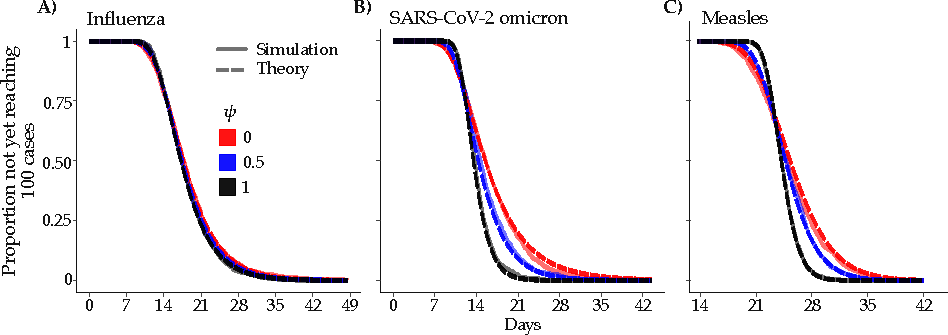
\includegraphics[width=\textwidth]{survival.pdf}
\caption{{\bf \boldmath Proportion of epidemics not yet reaching 100 infections for three pathogens.}  }
\label{fig:survival}
\end{figure}

% ////////////////////////////////////////////////////////////////////////////////////////////

\subsection{Narrow individual infectiousness profiles yield greater uncertainty in epidemic growth rate estimates}

Punctuated individual infectiousness profiles also make empirical estimates of the early-epidemic exponential growth rate $r$ more uncertain ({\bf Figure XX}). 

% ////////////////////////////////////////////////////////////////////////////////////////////

\subsection{Narrow biological infectiousness profiles interact with periodic contact patterns to generate overdispersion in secondary infections}

When each person has the same inherent infectiousness ($\nu_i \equiv R_0$) and contacts are uniform across individuals and over time ($c_i(t) \equiv \bar{c} = 1$), the timing of a person's secondary infections ($\xi_i(\tau)$) has no effect on the secondary infection distribution: every person produces a $\text{Poisson}(R_0)$-distributed number of infections. However, if contacts vary over time and/or across individuals, overdispersion may emerge as the interaction between $\xi_i$ and $c_i(t)$ produce variation in the realized individual reproduction number, $\nu_i^{\text{re}}$. 

The periodic contact model introduces temporal, but not interpersonal, variation in contacts. 

Similar results hold under the Gamma contact model, which introduces both temporal and interpersonal variation in contacts, but holds the population-average contact rate at $C(t) = 1$. 

%
\begin{equation}
	k = \frac{2}{A^2}\left(1 + \frac{\omega^2}{\beta^2}\right)^{\psi \alpha}
	\label{eq:k_periodic_main}
\end{equation}
%
where $A$ is the amplitude of the contact oscillation and $\omega$ is its angular frequency. Here, the prefactor $2/A^2$ sets the overall overdispersion scale, and the bracketed factor quantifies the failure of the biological profile's temporal window to average out the contact oscillation, with $(1 + \omega^2/\beta^2)^{-\psi\alpha}$ being exactly the squared characteristic function of the Gamma$(\psi\alpha, \beta)$ density at the contact frequency $\omega$. Since this factor is strictly increasing in $\psi$ for any $\omega > 0$, narrower biological profiles always produce more overdispersion in the presence of periodic contact variation. The effect disappears in the spike limit only if $\omega \rightarrow 0$ or $A \rightarrow 0$ (no temporal contact variation), and grows arbitrarily large in the smooth limit if $\omega/\beta$ is large (contact oscillations much faster than the profile window, so the profile averages them out). Simulations extend this result to heavier-tailed, non-periodic contact heterogeneity, for which the same mechanism holds qualitatively ({\bf Figure XX}).

% Even in large, well-mixed populations, stochasticity can durably impact the trajectory of an epidemic. One way this stochasticity enters is via a random time shift, where epidemics take a variable amount of time to reach the exponential growth phase \citep{morris_computation_2024}, leading to variation in the timing of the entire epidemic trajectory. Here, we address the question of how this time shift distribution depends on the shape of the individual infectiousness profile, holding all else equal. 

% Simulations confirm that narrower infectiousness profiles ($\psi \rightarrow 0$) yield more variable and later-shifted epidemic timings ({\bf Figure XX}, {\bf Supplementary Table Sxx}). Across 10,000 simulated epidemics in a population of size 1000 using SARS-CoV-2 omicron-like parameters, the median time to reach 100 infections was XX days for $\psi = 0$ (IQR: [XX, XX]) vs. XX days for $\psi = 1$ (IQR: [XX, XX]). The impact of $\psi$ on epidemic timing was lessened with lower $R_0$ (influenza-like parameters, median time to 100 infections: XX days for $\psi=0$ [IQR: XX, XX] vs. XX days for $\psi=1$ [IQR: XX, XX]) and increased with higher $R_0$ (measles-like parameters, median time to 100 infections: XX days for $\psi=0$ [IQR: XX, XX] vs. XX days for $\psi=1$ [IQR: XX, XX]). From another perspective: by day XX of the simulated epidemic under measles-like parameters, XX\% of the outbreaks with $\psi = 1$ had reached 100 infections, while only XX\% of the outbreaks with $\psi=0$ had reached 100 infections ({\bf Figure XX}). 

% These observations are confirmed by the underlying theory. The cumulative incidence over time, $Z(t)$, during the early exponential growth phase of an epidemic can be approximated as a deterministic exponential growth function with a random initial condition scaling factor $W$: 

% \begin{equation}
% 	Z(t) \approx W \cdot ce^{rt}
% \end{equation}

% with exponential growh rate $r$, and where $c$ is the mean-field initial condition (when $W = 1$). 

% With a change of variables, the cumulative incidence can be expressed as the same deterministic growht function with a random time shift $\varsigma$: 

% \begin{equation}
% 	Z(t) \approx c e^{r(t+\varsigma)}
% \end{equation}

% where 

% \begin{equation}
% 	\varsigma = \frac{\log W - \log E[W]}{r}
% \end{equation}

% Here, $E[W]$ is the initial condition and $r$ is the exponential growth rate, so $\varsigma \propto \log[W]$. 

% First, we consider the variance of the time shift, $Var[\varsigma]$. For ease of notation, we focus on $Var[W]$, noting that $Var[\varsigma]$ is monotonically related to $Var[W]$. It can be shown that {\bf Supplementary Text}

% \[ 
% Var[W] = m_2 + R_0^2 \rho^{2 \psi \alpha} [\rho_2^{(1-\psi)\alpha} - \rho^{2(1-\psi)\alpha}]
% \]

% which is maximized when $\psi = 0$ (the infectiousness profile is narrow) and becomes 0 when $\psi = 1$ (the infectiousness profile is maximally broad). (Can we say something about how this suggests that the variance of the time shift scales roughly linearly with $\psi$?)

% Next, we consider the typical time shift, which we obtain by studying the mode of the distribution of $W$. 

% Let $I_b(t)$ be the (stochastic) number of infections at time $t$ for a single epidemic realization, where the subscript ``b'' marks that it is a branching process. Let $I_d(t)$ be its mean-field deterministic counterpart. Then, we can approximate $I_b(t)$ as $I_d(t+\varsigma)$, {\it i.e.,} the branching process is approximately equal to the deterministic process with a random time shift. 

% The time shift is 

% \[ \varsigma = \frac{\log W - \log E[W]}{r}\]

% where $r$ is the epidemic's exponential growth rate and $W = \lim_{t \rightarrow \infty} W(t)$ is the limiting value of the rescaled branching process $W(t) = e^{-r t I_b(t)}$. The process $W(t)$ is well studied, and knowing its distribution fully determines the distribution of the time shift $\varsigma$. 

% The expectation of $W$ is equal to the initial condition ($E[W] = I_0$). For simplicity, we will assume $I_0 = 1$ throughout this section, though the findings can be easily extended to general initial conditions. Here, we assess the impact of the individual infectiousness profile's breadth, $\phi$, on (a) the variance of $W$ and (b) the mode of a Gamma approximation to W obtained via moment matching. 

% It can be shown that 

% \[ \text{Var}(W) = \frac{c^\alpha + \sigma^{(1-\psi) \alpha} - 1}{1 - c^\alpha} \]

% \noindent where $c$ depends on $R_0$ and $\alpha$ but not $\psi$. Thus, broad profiles ($\psi \rightarrow 1$) minimize $\text{Var}(W)$ and narrow profiles ($\psi \rightarrow 0$) maximize it. 

% We can approximate the distribution of $W$ using moment matching to a generalized Gamma distribution. With the Gamma-shaped individual infectiousness profiles, the moments have closed-form expressions. Using two-moment matching to a Gamma distribution, we find that 

% \[ \text{mode}_\varsigma = \frac{1}{r} \log(1 - \text{CV}^2_\text{cond})] \]

% Here, (description). Again, we see that the mode shifts later as $\psi \rightarrow 0$. 

% The theory aligns well with the simulations. Using generalized gamma distributions fit using moment matching to the first five moments of $W$, we get similar survival curves for the time to 100 infected ({\bf Figure XX}). 

% \subsection{Narrower individual infectiousness profiles yield greater uncertainty in epidemic growth rate estimates.}

% Based on simulations. 

% \subsection{Narrower biological infectiousness profiles interact with periodic contact patterns to generate overdispersion in secondary infections.}

% Closed-form solution: 

% \[ k = \frac{2}{\bar{c}^2}{A^2} \Bigl(1 + \frac{\omega^2}{r^2}\Bigr)^{\psi \alpha} = \frac{2}{\bar{c}^2}{A^2} \Bigl(1 + (\frac{z^*_{per}}{z_{per}})^2\Bigr)^{\psi \alpha} \]



% \begin{figure}[ht]
% \centering
% 
\includegraphics[width=.5\textwidth]{figures/stock.png}
% \caption{{\bf Impact of the individual infectiousness profile on epidemic timing.} Survival curves for time-to-100. growth rate estimate box-and-whiskers. Overdispersion/k vs psi heatmap.} 
% \label{fig:uncontrolled}
% \end{figure}


% Stepwise, smooth, and spike all yield the same mean dynamics
% Stepwise has higher extinction probability, explained by overdispersion
% Spike has later and more variable establishment properties, including time-to-n-infected and peak, and exponential growth rate is more variable. We can show this through simulations and through analytic approaches, following Morris' time shift ideas \citep{morris2024}

% With constant contacts, kappa doesn't affect extinction or overdispersion -- only growth timing

% but introduce time-varying contacts and suddenly kappa controls overdispersion

% Spike emphasizes variation in contacts, leading to overdispersion.


\section{The impact of punctuated infectiousness on outbreak interventions}

\subsection{Detection and isolation}

% Detection and isolation is more effective for punctuated kernels
% Detect-and-isolate policies shift the overall generation interval distribution in a way that depends on kappa -- leading to a partially self-defeating intervention.

\subsection{Contact tracing}

% Amidst all-same and kappa-variable scenarios, with tracing delays.

\subsection{Gathering size restrictions}

% More effective for smooth profiles, since they reduce mean transmission without losing the overdispersion that was suppressing outbreak probability for spiky profiles.


\section{Identifiability of punctuated infectiousness}

While the concentration of the individual infectiousness profile can impact how an epidemic unfolds, we lack frameworks for estimating it. Many approaches exist for estimating the generation interval, but there has not been a systematic approach developed to assess how individual infectiousness varies and to specify where on the continuum we sit---i.e., how much of the variation in the generation interval distribution is attributable to variation between individuals, and how much to variation in infection timing within individuals.


\clearpage

\section{Discussion}

Uncertain early exponential growth rate calculations feed into estimates of $R_0$ --- they are a critical ingredient for most $R_0$ estimation formulae. 

The superspreading mechanism introduced here is novel, and implies that some amount of superspreading cannot be traced {\it a priori} to the individual: there is no such thing as identifying superspreaders, since the superspreader in this case may not have any more inherent infectiousness or a greater number of contacts; instead, they were just infected at the wrong time. 

Accounting for the individual infectiousness profile is critical for anticipating the imapct of outbreak interventions. Simply calculating reductions in infectiousness is not enough: we get differences in overdispersion and the generation interval distribution that are sensitive to the punctuatedness of $a_i(\tau)$ and can lead to profoundly different epidemic dynamcis than a naive approach of simulating an equivalent epidemic without changing overdispersion or the generation interval distribution. 

Estiamting the shape of the individual infectiousness profile can be challenging given the need for precise estimates of time of infection and a good balance of depth and breadth of sampling. Fortunately, identifiability of the shape of $a_i(\tau)$ is better in situations where it matters most, \ie, when $R_0$ is high. 

{\bf Limitations.}

{\bf Concluding thoughts.}

\bibliographystyle{plainnat}
\bibliography{references}

\section*{Acknowledgements}

\section*{Funding}

\section*{Author contributions}


\clearpage
\appendix
\setcounter{equation}{0}
\setcounter{figure}{0}
\setcounter{table}{0}
\renewcommand{\theequation}{S\arabic{equation}}
\renewcommand{\thefigure}{S\arabic{figure}}
\renewcommand{\thetable}{S\arabic{table}}

\section*{Supplementary Information}

\subsection*{Supplementary Methods}

\subsubsection*{Parameter structure}

The punctuated Gamma model has four epidemiological parameters: the basic  reproduction number $R_0$, the early-epidemic growth rate $r$, and the two  parameters of the generation interval distribution, $\alpha$ (shape) and  $\beta$ (rate), which together determine the mean generation time  $\bar{g} = \alpha/\beta$. These four parameters are not all free: the  Euler--Lotka equation
%
\begin{equation}
	1  
	=R_0 \int_{\tau=0}^\infty e^{-r\tau } \frac{\beta^\alpha}{\Gamma(\alpha)} \tau^{\alpha-1} e^{-\beta \tau} d\tau
	= R_0 \left(\frac{\beta}{\beta + r}\right)^\alpha
	\label{eq:euler_lotka}
\end{equation}
%
provides one constraint among them, leaving three free parameters. We  choose to work with $(R_0, \bar{g}, \alpha)$ as the free parameters,  since each has a direct epidemiological interpretation. The rate parameter $\beta$ follows immediately from the  definition of the mean generation interval:
%
\begin{equation}
    \beta = \frac{\alpha}{\bar{g}},
\end{equation}
%
and the early-epidemic growth rate $r$ follows from the Euler--Lotka equation:
%
\begin{equation}
    r = \beta\left(R_0^{1/\alpha} - 1\right) 
      = \frac{\alpha}{\bar{g}}\left(R_0^{1/\alpha} - 1\right).
    \label{eq:r_from_params}
\end{equation}
%
The punctuation  parameter $\psi \in [0, 1]$ is the only remaining free parameter, and  it is the sole quantity that is not identifiable from population-level  epidemic data: since $A(\tau)$ is invariant across $\psi$ by  construction, the parameters $(R_0, \bar{g}, \alpha)$ can in principle  be estimated from the observed epidemic trajectory independently of  $\psi$. The consequences of varying $\psi$ while holding  $(R_0, \bar{g}, \alpha)$ fixed are therefore attributable purely to  changes in the individual-level temporal structure of infectiousness, with no confounding from changes in the population-level transmission  kernel.

\clearpage

\subsubsection*{Derivation of $E[\varsigma]$ and $\text{Var}[\varsigma]$}

{\bf Setup.} Following \citet{morris_computation_2024}, we describe the cumulative infections during the early-epidemic exponential growth phase as a branching process, $Z(t)$. Let $r$ be the epidemic's exponential growth rate; then, as $t \rightarrow \infty$, $e^{-rt} Z(t) \rightarrow W$ almost surely, where $W$ is a random variable that effectively scales the branching process' initial condition, capturing stochastic fluctuations in the early-epidemic process. We denote this convergence as $Z(t) \approx W \cdot e^{rt}$. 

% Here, $r$ is the early-epidemic exponential growth rate and $W$ is a random variable that effectively scales the branching process' initial condition, capturing stochastic fluctuations in the early-epidemic process. 

With a change of variables, we can translate $W$ into a random initial time shift: 
%
\begin{equation}
	Z(t) \approx e^{r (t + \varsigma)} \qquad \text{where} \qquad \varsigma = \frac{\log W - \log E[W]}{r} = \frac{\log W}{r}
\end{equation}
%
when $I_0 = E[W] = 1$ (\ie, when the epidemic is seeded with a single infectious person). Our goal is to determine how $E[\varsigma]$ and $\text{Var}[\varsigma]$ depend on the punctuation parameter $\psi$. To achieve this, we begin by examining the distribution of $W$. 

\noindent {\bf \boldmath Approximating the distribution of $W$.} First, we note that the distribution of $W$ consists of a point mass at 0 with mass $q$ (the probability of epidemic extinction), combined with a smooth density with positive support. The point mass translates into a time shift of $\varsigma = \log(0) / r = -\infty$, corresponding to an epidemic that never establishes. Thus, we restrict our attention to $W | \text{surv}$ and $\varsigma | \text{surv}$, that is, $W$ and $\varsigma$ conditioned on epidemic survival. 

To approximate the distribution of $W|\text{surv}$, we use a $\text{Gamma}(k, \lambda)$ distribution matched to the first two moments. This is a version of the five-moment-matching approach described by \cite{morris_computation_2024}, simplified for analytic tractability. Specifically, we let  
\begin{equation}
	k = \frac{E[W|\text{surv}]^2}{\text{Var}[W|\text{surv}]} \qquad \text{and} \qquad \lambda = \frac{E[W|\text{surv}]}{\text{Var}[W|\text{surv}]}
	\label{eq:k_and_lambda}
\end{equation}
Our task is now to compute $E[W|\text{surv}]$ and $\text{Var}[W|\text{surv}]$. 

\noindent {\bf \boldmath Deriving $E[W|\text{surv}]$.} We note that 
\begin{equation}
E[W] = E[W|\text{surv}] P(\text{surv}) + E[W|\text{extinct}] P(\text{extinct}) = E[W | \text{surv}] \cdot p
\label{eq:p_explanation}
\end{equation}
since $E[W|\text{extinct}] = 0$, and where $p = 1-q$ is the probability of epidemic survival. Thus,
\begin{equation}
\boxed{E[W|\text{surv}] = \frac{1}{p}}
\end{equation}
\begin{center}
{\it [for plugging into expressions for $k$ and $\lambda$, Eq.~\ref{eq:k_and_lambda}]} \\ 
\end{center} 
under our assumption that $E[W] = 1$. 

\noindent {\bf \boldmath Deriving $\text{Var}[W|\text{surv}]$.} The derivation for $\text{Var}[W]$ is somewhat more involved. Recall the Gamma time-shift model, where an infectious person produces $\chi_i \sim \text{Poisson}(R_0)$ secondary infections distributed at times $\tau_j = l_i+ \epsilon_j,\, j\in \{1, \dots, \chi_i\}$ and 
\begin{equation}
l_i \sim \text{Gamma}((1-\psi) \alpha, \beta), \qquad \epsilon_j \sim \text{Gamma}(\psi \alpha, \beta)
\end{equation}
This ensures that a random secondary infection time $\tau$ is distributed according to the generation interval distribution $g(\tau)$, \ie,
\begin{equation}
	\tau \sim \text{Gamma}(\alpha, \beta)
\end{equation}
For notational convenience, we introduce 
\begin{equation}
	E[e^{-c r \tau}] = \int_0^\infty e^{-cr\tau} \frac{\beta^\alpha}{\Gamma(\alpha)} \tau^{\alpha-1} e^{-\beta \tau}\, d\tau
	 = \Bigl(\frac{1}{1 + cz}\Bigr)^\alpha := \rho_c^\alpha
\end{equation}
that is, 
\begin{equation}
\boxed{\rho_c = \frac{1}{1+cz}}
\end{equation}
\begin{center}
{\it [for notational convenience]} \\ 
\end{center}
where $z = r/\beta = r \bar{g} / \alpha = R_0^{1/\alpha} - 1$, a dimensionless quantity that simplifies expressions and allows one to easily plug in different combinations of epidemiological parameters. Here, $\bar{g}$ is the mean of the generation interval distribution $g(\tau)$, and $c$ is a positive integer. The final expression, $z = R_0^{1/\alpha} - 1$, comes from the Euler-Lotka equation \citep{wallinga_how_2007}: 
\begin{equation}
1 = R_0 E[e^{-r \tau}] = R_0 \rho_1^\alpha 
= R_0 \Bigl(\frac{1}{1+z}\Bigr)^\alpha
\label{eq:euler_lotka}
\end{equation}
% \begin{equation}
% 1 = R_0 E[e^{-r \tau}] = R_0 \int_0^\infty e^{-r \tau} \frac{\beta^\alpha}{\Gamma(\alpha)} \tau^{-\alpha-1} e^{-\beta \tau}\, d\tau
% = R_0 \Bigl(\frac{1}{1+z}\Bigr)^\alpha
% \end{equation}
and solving for $z$. 


Next, we introduce the distributional fixed point equation, which is a standard starting point for computing moments of $W$. This equation exploits the self-similarity of the branching process, in which an epidemic initiated by a single individual is, in distribution, a scaled and time-shifted copy of the whole epidemic. At large $t$, the epidemic seeded by the index case $i$ consists of the downstream epidemics caused by their offspring $j$, which have grown approximately to size $Z_j(t) = W_j e^{r(t - \tau_j)}$. That is, 
%
\[
	Z(t) \approx \sum_{j=1}^{\chi_i} W_j e^{rt} e^{-r \tau_j}
\]
Multiplying through by $e^{-rt}$: 
%
\[  W \overset{d}{=} \sum_{j=1}^{\chi_i} e^{-r \tau_j} W_j \]

We now use this expression to calculate $\text{Var}[W]$. Since randomness enters through both $W$ and $\tau$, we first condition on the number of offspring and their infection times, $\tau_\bullet = \{ \chi_i, \tau_1, \tau_2, \dots, \tau_{\chi_i} \}$, using the law of total variance: 
%
\[ \text{Var}[W] = E[\text{Var}\Bigl[\sum_j e^{-r \tau_j} W_j | \tau_\bullet\Bigr]] + \text{Var}[E\Bigl[\sum_j e^{-r \tau_j} W_j | \tau_\bullet\Bigr]] \]
\[
=E\Bigl[ \sum_j e^{-2r\tau_j}  \cdot \text{Var}[W] \Bigr] + 
\text{Var} \Bigl[\sum_j e^{-r \tau_j} \cdot E[W] \Bigr]
\]
\[
= E\Bigl[\sum_j e^{-2 r \tau_j}\Bigr] \cdot \text{Var}[W] + 
(E[W])^2 \cdot \text{Var}\Bigl[\sum_j e^{-r \tau_j}\Bigr]
\]
%
Since $E[W] = I_0 = 1$, we have 
\[
	\text{Var}[W] = \text{Var}[W] E\Bigl[\sum_j e^{-2 r \tau_j}\Bigr] + \text{Var}\Bigl[\sum_j e^{-r \tau_j}\Bigr]
\]
Solving for $\text{Var}[W]$, 
\[
	\text{Var}[W] = \frac{\text{Var}[\sum_j e^{-r \tau_j}]}{1 - E[\sum_j e^{-2 r \tau_j}]}
\]
To simplify the denominator, note that 
\[ 
E\Bigl[\sum_{j=1}^{\chi_i} e^{-2 r \tau_j}\Bigr] = E[\chi_i] E[e^{-2 r \tau_j}]
 = R_0 E[e^{-2 r \tau_j}]
 % = R_0 \Bigl( \frac{\beta}{\beta + 2r}\Bigr )^\alpha 
 = R_0 \rho_2^\alpha 
 \]
Thus, the variance expression simplifies to 
\[
	\text{Var}[W] = \frac{\text{Var}[\sum_j e^{-r \tau_j}]}{1 - R_0 \rho_2^\alpha}
\]
Next, we examine the numerator: 
\[
	\text{Var}[\sum_j e^{-r \tau_j}] = E[(\sum_j e^{-r \tau_j})^2] - E[\sum_j e^{-r \tau_j}]^2 = E[(\sum_j e^{-r \tau_j})^2] - 1
\]
where the last step follows from the Euler-Lotka equation (Eq.~\ref{eq:euler_lotka}). 
% The second term is (R_0 \frac{1}{1+z})
% \[
% 	\text{Var}[\sum_j e^{-r \tau_j}] = E[(\sum_j e^{-r \tau_j})^2] - E[\sum_j e^{-r \tau_j}]^2 = E[(\sum_j e^{- r \tau_j})^2] - 1
% \]
Then, 
\[
	E[(\sum_j e^{- r \tau_j})^2] = E[\sum_j e^{-2 r \tau_j}] + E[\sum_{j \neq k} e^{-r (\tau_j + \tau_k)}]
\]
\[= R_0 \rho_2^\alpha + E[\chi_i (\chi_i - 1)] E[e^{-r \tau_j} e^{-r \tau_k}]\]
\[= R_0 \rho_2^\alpha + R_0^2 E[e^{-r \tau_j} e^{-r \tau_k}]\]
Here, the $\chi_i (\chi_i - 1)$ term enters because there are this many terms in the sum over $j \neq k$. Also, 
\[
E[\chi_i (\chi_i - 1)] = E[\chi_i^2] - E[\chi_i] = \text{Var}[\chi_i] + E[\chi_i]^2 - E[\chi_i] = R_0 + R_0^2 - R_0 = R_0^2
\]
under the assumption that $\chi_i \sim \text{Poisson}(R_0)$. 

Since $\tau_j = l_i + \epsilon_j$, and since $l_i$, $\epsilon_j$, and $\epsilon_k$ are independent, 
\[ E[e^{-r \tau_j} e^{-r \tau_k}]  = E[e^{-2r l_i} e^{-r \epsilon_j} e^{-r \epsilon_k}] = E[e^{-2r l_i}] (E[e^{-r \epsilon}])^2 = \rho_2^{(1-\psi)\alpha} \cdot \rho _1^{2 \psi \alpha}\]
Finally, we can assemble $\text{Var}[W]$: 
\[
	\text{Var}[\sum_j e^{-r \tau_j}] = R_0 \rho_2^\alpha + R_0^2 \rho_2^{(1-\psi)\alpha} \rho_1^{2 \psi \alpha} - 1
\]
and thus, substituting in the $z$ expressions for $\rho_1$ and $\rho_2$ and noting $R_0 = (1 + z)^\alpha$, we obtain
\begin{equation}
	\text{Var}[W] = \frac{
		\Bigl(\frac{1 + z}{1 + 2z}\Bigr)^\alpha + \Bigl(\frac{(1 + z)^2}{1 + 2z}\Bigr)^{(1-\psi) \alpha} - 1
	}{
		1 - \Bigl(\frac{1 + z}{1 + 2z}\Bigr)^\alpha
	} := 
	\frac{\sigma_1^\alpha + \sigma_2^{(1-\psi)\alpha} - 1}{1 - \sigma_1^\alpha}
\end{equation}
where $\sigma_c = \frac{(1 + z)^c}{1 + 2z}$ for positive integer $c$. 

  Last, we note that $E[W^n|\text{surv}] = E[W^n]/p$
  (by the same logic as in Eq.~\ref{eq:p_explanation}), so
  \begin{align}
      \text{Var}[W | \text{surv}]
      &= E[W^2|\text{surv}] - E[W|\text{surv}]^2 = \frac{1}{p} E[W^2] - \frac{1}{p^2} E[W]^2 \\ 
      &= \boxed{\frac{1}{p} (1 + \text{Var}[W]) - \frac{1}{p^2}}
  \end{align}  
% Last, we note that, by the same logic as in Eq.~\ref{eq:p_explanation}, 
% \begin{equation}
% 	\text{Var}[W | \text{surv}] = \frac{1}{p} \cdot \frac{
% 		\Bigl(\frac{1 + z}{1 + 2z}\Bigr)^\alpha + \Bigl(\frac{(1 + z)^2}{1 + 2z}\Bigr)^{(1-\psi) \alpha} - 1
% 	}{
% 		1 - \Bigl(\frac{1 + z}{1 + 2z}\Bigr)^\alpha
% 	}
% \end{equation}
\begin{center}
{\it [for plugging into expressions for $k$ and $\lambda$, Eq.~\ref{eq:k_and_lambda}]}
\end{center}

\noindent {\bf \boldmath Expressions for $k$ and $\lambda$.} Combining the previous derivations and plugging into Eq.~\ref{eq:k_and_lambda} gives 
\begin{equation}
\boxed{k = \frac{1 - \sigma_1^\alpha}{p \sigma_2^{(1 - \psi)\alpha} - 1 + \sigma_1^\alpha},
\qquad
\lambda = p k }
\end{equation}
\begin{center}
	{\it [Parameters of the moment-matched Gamma distribution for W]}
\end{center}

\noindent {\bf \boldmath Deriving the approximate density of $\varsigma$.} Let $f_W(x)$ be the Gamma-distributed approximate density of $W$: 
\begin{equation}
	f_W(x) = \frac{\lambda^k}{\Gamma(k)} x^{k-1} e^{-\lambda x}
\end{equation}
Since $\varsigma = \frac{1}{r} \log W$, we have $W = e^{r \varsigma}$, or, in terms of the arguments of the density functions, $x = e^{r s}$. By the change of variables formula, the density of $\varsigma$ is 
\begin{equation}
f_\varsigma(s) = f_W(e^{rs}) |\frac{dw}{ds}| = 
\frac{\lambda^k}{\Gamma(k)} e^{rs(k-1)} e^{-\lambda e^{rs}} r e^{rs} = \frac{r \lambda^k}{\Gamma(k)} e^{rsk} e^{-\lambda e^{rs}}
\label{eq:varsigma_dist}
\end{equation}
By taking the logarithm, differentiating with respect to $s$, and setting equal to 0, we can determine the mode of the distribution: 
\begin{equation}
	\boxed{\text{Mode}[\varsigma] = \frac{1}{r} \log \Bigl(\frac{k}{\lambda}\Bigr) = \frac{1}{r} \log \frac{1}{p}}
	\label{eq:varsigma_mode}
\end{equation}
\begin{center}
	{\it [Mode of the time shift distribution]}
\end{center}
Thus, the modal time shift depends on the epidemic growth rate $r$ and the establishment probability $p$ (and thus the reproduction number $R_0$), but not on the punctuation parameter $\psi$. 


\noindent {\bf \boldmath Deriving $E[\varsigma]$.} 
It would be possible to derive $E[\varsigma]$ directly from Eq.\ref{eq:varsigma_dist}, but there is a more direct route: since $W \sim \text{Gamma}(k,\lambda)$ and $\varsigma = \frac{1}{r} \log(W)$, it follows that 
\begin{equation}
	E[\varsigma] = \frac{1}{r}(\Psi^{(0)}(k) - \log \lambda)
\end{equation}
where $\Psi^{(0)}(k)$ is the digamma function evaluated at $k$. Plugging in $\lambda = pk$: 
\begin{equation}
\boxed{E[\varsigma] = \frac{\log(1/p)}{r} + \frac{\Psi^{(0)}(k) - \log(k)}{r}}
\end{equation}
\begin{center}
	{\it [Expected value of the time shift distribution]}
\end{center}
The first term is $\text{Mode}[\varsigma]$ (Eq.~\ref{eq:varsigma_mode}), and is independent of the punctuation parameter $\psi$. The second term is a $\psi$-dependent adjustment that is: 
\begin{enumerate}
	\item {\bf  Strictly negative.} {\it Proof:} Let $G \sim \text{Gamma}(k,1)$. Then, $E[G] = k$ and $E[\log G] = \Psi^{(0)}(k)$. By Jensen's inequality, since $\log$ is strictly concave, 
	\[\Psi^{(0)}(k) = E[\log G] < \log(E[G]) = \log k \]
	Thus, $\bigl(\Psi^{(0)}(k) - \log(k)\bigr)/r < 0$. 
	\item {\bf \boldmath Strictly increasing (less negative) in $\psi$.} {\it Proof:} Consider 
	\[\frac{d}{dk} \bigl[ \Psi^{(0)}(k) - \log k \bigr] = 
	\frac{d}{dk} \Biggl[ \int_0^\infty \Bigl(\frac{e^{-t}}{t} - \frac{e^{-kt}}{1 - e^{-t}}\Bigr) dt \Biggr] - \frac{1}{k} 
	= \int_0^\infty \frac{t e^{-k t }}{1 - e^{-t}}\, dt  - \frac{1}{k}
	\]
	Note that $1 - e^{-t} < t$ for $t > 0$, and thus $\frac{t}{1 - e^{-t}} > 1$. So, 
	\[  
	\int_0^\infty \frac{t e^{-kt}}{1 - e^{-t}} > \int_0^\infty e^{-kt} = \frac{1}{k}
	 \]
	 So, 
	 \[\frac{d}{dk} \bigl[ \Psi^{(0)}(k) - \log k \bigr] > 0 \]
	 and thus $(\Psi^{(0)}(k) - \log k)/r$ is increasing in $k$. \\ 
	 Next, we note that $k$ is increasing in $\psi$. The only $\psi$-dependent quantity in $k$ (Eq.\ref{eq:k_and_lambda}) is $\sigma_2^{(1-\psi)\alpha}$, which shows up in the denominator. Since
	 \[\sigma_2 = \frac{(1 + z)^2}{(1 + 2z)} = 1 + \frac{z^2}{1 + 2z} > 1 \quad \text{ for  } z > 0\]
	 the term is maximized when $\psi = 0$ and minimized when $\psi = 1$. Thus, $k$ is minimized when $\psi = 0$ and maximized when $\psi = 1$ --- \ie, $k$ is increasing in $\psi$. 
\end{enumerate}

\noindent Together, these observations demonstrate that the expected time shift sits later than the modal time shift (\ie, the time shift is left-skewed; Observation 1), and the expected time shift moves increasingly later as $a_i(\tau)$ becomes more punctuated (Observation 2). 

\noindent {\bf \boldmath Deriving $\text{Var}[\varsigma]$.} Following again from the properties of $\log W$ where $W$ is $\text{Gamma}(k, \lambda)$-distributed, 
\begin{equation}
	\boxed{\text{Var}[\varsigma] = \frac{1}{r^2} \Psi^{(1)}(k)}
\end{equation}
\begin{center}
	{\it [Variance of the time shift distribution]}
\end{center}
where $\Psi^{(1)}(k)$ is the trigamma function. The trigamma function is strictly decreasing in $k$, since 
\begin{equation}
\frac{d}{dk} \Psi^{(1)}(k) =  \frac{d}{dk }\sum_{n=0}^\infty \frac{1}{(k+n)^2} = 
-2 \sum_{n=0}^\infty \frac{1}{(k + n)^3}
\end{equation}
which is strictly negative when $k > 0$. Thus, $\psi \rightarrow 0$ (punctuated profiles) $\Rightarrow$ $k$ decreasing $\Rightarrow$ $\text{Var}[\varsigma]$ increasing, \ie, more punctuated profiles increase the variance of the time shift. 

\noindent {\bf Summary.} In this section, we derived properties of the random time shift $\varsigma$ by relying on a branching process approximation to the early-epidemic exponential growth phase. When conditioning on epidemic survival, we demonstrated that the time shift becomes increasingly later in expectation and more variable as the individual infectiousness profile $a_i(\tau)$ becomes more punctuated ($\psi \rightarrow 0$).

\clearpage

\subsubsection*{Generality beyond the time-shifted Gamma model}

The preceding derivation used the time-shifted Gamma model and a Gamma-distributed generation interval. Here, we show that the core result --- punctuated profiles increase the variance of early-epidemic timing --- holds for \emph{any} non-degenerate generation interval distribution (\ie, any distribution with positive variance, as opposed to a degenerate distribution concentrated on a single point). The argument rests only on the additive splitting $\tau_j = l_i + \varepsilon_j$ (shared shift plus independent jitter) and the Cauchy-Schwarz inequality.

\noindent {\bf Setup.} Let $g$ be an arbitrary generation interval distribution with Laplace transform $M_g(s) = E[e^{-s\tau}]$, so the Euler-Lotka equation gives $R_0 M_g(r) = 1$. Each index case's offspring share a common latent shift $l_i$ and receive independent jitter $\varepsilon_j$, so $\tau_j = l_i + \varepsilon_j$ with the marginal distribution of $\tau_j$ equal to $g$. The distributions of $l$ and $\varepsilon$ are arbitrary, subject only to $M_l \cdot M_\varepsilon = M_g$.

\noindent {\bf \boldmath Model-free $\text{Var}[W]$ formula.} The law-of-total-variance derivation proceeds identically to the Gamma case. The only splitting-dependent step is the cross-term for $j \neq k$:
\[
E[e^{-r \tau_j} e^{-r \tau_k}] = E[e^{-2rl}] (E[e^{-r\varepsilon}])^2 = M_l(2r) \cdot M_\varepsilon(r)^2
\]
Using $M_l(2r) = M_g(2r) / M_\varepsilon(2r)$, this becomes $M_g(2r) \cdot Q$, where
\begin{equation}
	Q := \frac{M_\varepsilon(r)^2}{M_\varepsilon(2r)}
	\label{eq:Q_def}
\end{equation}
Assembling the full variance formula (with $A := R_0 M_g(2r)$):
\begin{equation}
	\text{Var}[W] = \frac{A(1 + R_0 Q) - 1}{1 - A}
	\label{eq:var_W_general}
\end{equation}
Here, $A$ depends only on $g$ and not on the splitting, and $Q$ is the \emph{only} place the splitting enters. Since Eq.~\ref{eq:var_W_general} is affine in $Q$ with positive slope $R_0 A / (1-A)$, $\text{Var}[W]$ is strictly increasing in $Q$.

\noindent {\bf Three properties of $Q$.}

\begin{enumerate}
	\item $Q \leq 1$, with equality if and only if $\varepsilon$ is degenerate (maximum punctuation).

	{\it Proof:} By the Cauchy-Schwarz inequality applied to $X = e^{-r\varepsilon}$:
	\[M_\varepsilon(2r) = E[X^2] \geq (E[X])^2 = M_\varepsilon(r)^2\]
	so $Q = M_\varepsilon(r)^2 / M_\varepsilon(2r) \leq 1$. Equality holds if and only if $X$ is almost surely constant, \ie, $\varepsilon$ is degenerate. $\blacksquare$

	\item $Q$ is multiplicative under convolution: if $\varepsilon_2 \overset{d}{=} \varepsilon_1 + \delta$ with $\delta$ independent, then $Q_2 = Q_1 \cdot Q_\delta \leq Q_1$, with strict inequality if $\delta$ is non-degenerate.

	{\it Proof:} $M_{\varepsilon_2}(s) = M_{\varepsilon_1}(s) \cdot M_\delta(s)$, so $Q_2 = Q_1 \cdot M_\delta(r)^2 / M_\delta(2r) = Q_1 \cdot Q_\delta$, and $Q_\delta \leq 1$ by Property 1. $\blacksquare$

	\item The spike-vs-smooth gap in $\text{Var}[W]$ is strictly positive for any non-degenerate $g$.

	{\it Proof:} For the spike ($\varepsilon = 0$), $Q_\text{spike} = 1$. For the smooth ($\varepsilon = \tau$, $l = 0$), $Q_\text{smooth} = M_g(r)^2 / M_g(2r) = 1 / (R_0^2 M_g(2r)) = 1/(R_0 A)$. The gap is
	\[
	\text{Var}[W]_\text{spike} - \text{Var}[W]_\text{smooth} = \frac{R_0 A (1 - Q_\text{smooth})}{1 - A} = \frac{R_0 A - 1}{1 - A}
	\]
	Since $R_0 A = R_0^2 M_g(2r) \geq R_0^2 M_g(r)^2 = 1$ by the Cauchy-Schwarz inequality applied to $X = e^{-r\tau}$, with strict inequality for non-degenerate $g$, the gap is strictly positive. $\blacksquare$
\end{enumerate}

\noindent {\bf Monotonicity for parameterized families.} For a one-parameter family of splittings $\varepsilon_\psi$ with $\varepsilon_0 = 0$ (spike) and $\varepsilon_1 = \tau$ (smooth), if the family is ordered by convolution --- meaning $\varepsilon_{\psi_2} \overset{d}{=} \varepsilon_{\psi_1} + \delta$ for some independent $\delta \geq 0$ whenever $\psi_2 > \psi_1$ --- then $Q(\psi)$ is strictly decreasing and $\text{Var}[W](\psi)$ is strictly decreasing in $\psi$. The time-shifted Gamma model satisfies this ordering, since $\text{Gamma}(\psi_2 \alpha, \beta) \overset{d}{=} \text{Gamma}(\psi_1 \alpha, \beta) + \text{Gamma}((\psi_2 - \psi_1) \alpha, \beta)$, but any infinitely divisible generation interval distribution admits such a family.

\noindent {\bf Implications for the full chain.} Combined with the model-free conditioning step ($\text{Var}[W|\text{surv}] = (1 + \text{Var}[W])/p - 1/p^2$, which increases in $\text{Var}[W]$) and the Gamma-approximation results above, the full chain holds for general $g$:
\begin{center}
\begin{tabular}{ccccccc}
	More punctuation & $\Rightarrow$ & higher $Q$ & $\Rightarrow$ & higher $\text{Var}[W]$ & $\Rightarrow$ & lower $k$ \\
	& & {\scriptsize (Cauchy-Schwarz)} & & {\scriptsize (Eq.~\ref{eq:var_W_general})} & & {\scriptsize (Eq.~\ref{eq:k_and_lambda})} \\[6pt]
	& $\Rightarrow$ & more negative $E[\varsigma]$ & and & higher $\text{Var}[\varsigma]$ \\
	& & {\scriptsize (digamma monotonicity)} & & {\scriptsize (trigamma monotonicity)} \\
\end{tabular}
\end{center}
The first two links are model-free: the only assumption is that $g$ is non-degenerate. The final link --- from $\text{Var}[W]$ to properties of $\varsigma = (\log W)/r$ --- requires a distributional assumption, because moments of $W$ do not uniquely determine moments of $\log W$. The Gamma moment-matching approximation serves this role: given $E[W|\text{surv}]$ and $\text{Var}[W|\text{surv}]$, it provides a complete distribution from which $E[\varsigma]$ and $\text{Var}[\varsigma]$ can be computed in closed form via the digamma and trigamma functions. Without this (or an analogous) approximation, the qualitative direction is still supported by Jensen's inequality --- which guarantees $E[\varsigma|\text{surv}] < \log(1/p)/r$ for any distribution of $W|\text{surv}$, with the gap increasing when the distribution becomes more dispersed in the sense of convex order --- but the specific quantitative expressions would not apply.











% \noindent To complete the argument, we show that $k$ is increasing in $\psi$. Recall from Eq.~\ref{eq:k_and_lambda} that
% \[
% k = \frac{1 - \sigma_1^\alpha}{p\, \sigma_2^{(1-\psi)\alpha} + \sigma_1^\alpha - 1}
% \]
% The numerator does not depend on $\psi$. In the denominator, the only $\psi$-dependent term is $\sigma_2^{(1-\psi)\alpha}$, whose derivative with respect to $\psi$ is
% \[
% \frac{d}{d\psi} \sigma_2^{(1-\psi)\alpha} = -\alpha \log(\sigma_2) \cdot \sigma_2^{(1-\psi)\alpha} < 0
% \]
% since $\sigma_2 = (1+z)^2/(1+2z) = 1 + z^2/(1+2z) > 1$ for $z > 0$. Thus, the denominator is strictly decreasing in $\psi$, and $k$ (a positive constant divided by a decreasing positive function) is strictly increasing in $\psi$.

% \noindent {\bf Summary.} Combining the three results above: as $\psi$ decreases (more punctuated infectiousness), $k$ decreases, making the Jensen gap $(\Psi^{(0)}(k) - \log k)/r$ more negative, and thus $E[\varsigma]$ more negative --- meaning epidemics reach the establishment threshold earlier, on average.

% secondary infection time are distributed according to the generation interval distribution $g(\tau)$, \ie, $\tau_j \sim \text{Gamma}(\alpha, \beta)$


% For notational convenience, we introduce 
% \begin{equation}
% 	\rho_c = E[e^{-c r \tau}] = 
% \end{equation}





% Our first step is to approximate the distribution of $W$, conditional on epidemic survival, with a $\text{Gamma}(k, \lambda)$ distribution by matching the first two moments. Specifically, we set
% % \begin{equation}
% % 	k = \frac{}
% % \end{equation}


% Our first step is to approximate the distribution of $W$, which we denote $f_W(x)$, with an approximate distribution $\tilde{f}_W(x)$ that follows a $\text{Gamma}(k,\lambda)$ distribution. 





% \clearpage


% \subsubsection*{Derivation of $\text{Var}[W]$}

% For a branching process $Z(t)$ conditional on non-extinction, $e^{-rt} Z(t) \rightarrow W$ almost surely as $t \rightarrow \infty$. Here, $r$ is the early-epidemic exponential growth rate and $W$ is a random variable that effectively scales the branching process' initial condition, capturing stochastic fluctuations in the early-epidemic process. 

% With a change of variables, we can translate $W$ into a random initial time shift: 
% %
% \begin{equation}
% 	\varsigma = \frac{\log W - \log E[W]}{r} = \frac{\log W}{r}
% \end{equation}
% %
% when $I_0 = E[W] = 1$. Our goal is to understand how $\text{Var}[\varsigma]$ depends on the punctuation parameter $\psi$. Since $\varsigma$ and $W$ are monotonically related, we can derive an expression for $\text{Var}[W]$ and will interpret its implications for $\text{Var}[\varsigma]$ at the end. 

% To start, we consider an index case $i$ infected at time $t = 0$ who produces $\chi_i \sim \text{Poisson}(R_0)$ offspring. Under the Gamma time-shift model, the offspring $j$ from this index case are infected at times $\tau_j = l_i + \epsilon_j$, where $l_i$ is person $i$'s latent period and $\epsilon_j$ is the additional lag between $l_i$ and person $j$'s infection time, with 
% %
% \[l_i \sim \text{Gamma}((1-\psi)\alpha, \beta), \qquad \epsilon_j \sim \text{Gamma}(\psi \alpha, \beta) \]
% %
% This ensures that the population-level generation interval distribution is
% %
% \[ g(\tau) \sim \text{Gamma}(\alpha, \beta) \]
% %
% We can define some useful quantities that will arise later in the derivation. First, from the Euler-Lotka equation under $g(\tau)$ \citep{wallinga_how_2007}:, 
% %
% \[1 = R_0 \int_{\tau=0}^\infty e^{-r\tau } \frac{\beta^\alpha}{\Gamma(\alpha)} \tau^{\alpha-1} e^{-\beta \tau} d\tau\]
% %
% which simplifies to 
% %
% \[ 1 = R_0 \Bigl( \frac{\beta}{\beta+r }\Bigr )^\alpha = R_0 \Bigl(\frac{1}{1+z}\Bigr)^\alpha\]
% %
% where  $z = r/\beta = r \bar{g} / \alpha = R_0^{1/\alpha} - 1$, a dimensionless quantity that simplifies expressions and allows one to easily plug in different combinations of epidemiological parameters. Here, $\bar{g}$ is the mean of the generation interval distribution $g(\tau)$. 

% Next, we define 
% %
% \[ \rho_k =  (E[e^{-k r \tau}])^{1/\alpha} = \frac{\beta}{\beta + k r}  = \frac{1 }{1 + kz}\]
% This allows us to re-write the Euler-Lotka equation: 
% %
% \[ 1 = R_0 \rho_1^\alpha \]

% Next, we introduce the distributional fixed point equation, which is a standard starting point for computing moments of $W$. This equation exploits the self-similarity of the branching process, in which an epidemic initiated by a single individual is, in distribution, a scaled and time-shifted copy of the whole epidemic. At large $t$, the epidemic seeded by the index case $i$ consists of the downstream epidemics caused by their offspring $j$, which have grown approximately to size $Z_j(t) = W_j e^{r(t - \tau_j)}$. That is, 
% %
% \[
% 	Z(t) \approx \sum_{j=1}^{\chi_i} W_j e^{rt} e^{-r \tau_j}
% \]
% Multiplying through by $e^{-rt}$: 
% %
% \[  W \overset{d}{=} \sum_{j=1}^{\chi_i} e^{-r \tau_j} W_j \]

% We now use this expression to calculate $\text{Var}[W]$. Since randomness enters through both $W$ and $\tau$, we first condition on $\tau_j$ using the law of total variance: 
% %
% \[ \text{Var}[W] = E[\text{Var}\Bigl[\sum_j e^{-r \tau_j} W_j | \tau_j\Bigr]] + \text{Var}[E\Bigl[\sum_j e^{-r \tau_j} W_j | \tau_j\Bigr]] \]
% \[
% =E\Bigl[ \sum_j e^{-2r\tau_j}  \cdot \text{Var}[W] \Bigr] + 
% \text{Var} \Bigl[\sum_j e^{-r \tau_j} \cdot E[W] \Bigr]
% \]
% \[
% = E\Bigl[\sum_j e^{-2 r \tau_j}\Bigr] \cdot \text{Var}[W] + 
% (E[W])^2 \cdot \text{Var}\Bigl[\sum_j e^{-r \tau_j}\Bigr]
% \]
% %
% Since $E[W] = I_0 = 1$, we have 
% \[
% 	\text{Var}[W] = \text{Var}[W] E\Bigl[\sum_j e^{-2 r \tau_j}\Bigr] + \text{Var}\Bigl[\sum_j e^{-r \tau_j}\Bigr]
% \]
% Solving for $\text{Var}[W]$, 
% \[
% 	\text{Var}[W] = \frac{\text{Var}[\sum_j e^{-r \tau_j}]}{1 - E[\sum_j e^{-2 r \tau_j}]}
% \]
% To simplify the denominator, note that 
% \[ 
% E\Bigl[\sum_{j=1}^{\chi_i} e^{-2 r \tau_j}\Bigr] = E[\chi_i] E[e^{-2 r \tau_j}]
%  = R_0 E[e^{-2 r \tau_j}]
%  % = R_0 \Bigl( \frac{\beta}{\beta + 2r}\Bigr )^\alpha 
%  = R_0 \rho_2^\alpha 
%  \]
% Thus, the variance expression simplifies to 
% \[
% 	\text{Var}[W] = \frac{\text{Var}[\sum_j e^{-r \tau_j}]}{1 - R_0 \rho_2^\alpha}
% \]
% The denominator does not depend on $\psi$, so we proceed by examining the numerator: 
% \[
% 	\text{Var}[\sum_j e^{-r \tau_j}] = E[(\sum_j e^{-r \tau_j})^2] - E[\sum_j e^{-r \tau_j}]^2 = E[(\sum_j e^{- r \tau_j})^2] - 1
% \]
% Then, 
% \[
% 	E[(\sum_j e^{- r \tau_j})^2] = E[\sum_j e^{-2 r \tau_j}] + E[\sum_{j \neq k} e^{-r (\tau_j + \tau_k)}]
% \]
% \[= R_0 \rho_2^\alpha + E[\chi_i (\chi_i - 1)] E[e^{-r \tau_j} e^{-r \tau_k}]\]
% \[= R_0 \rho_2^\alpha + R_0^2 E[e^{-r \tau_j} e^{-r \tau_k}]\]
% Here, the $\chi_i (\chi_i - 1)$ term enters because there are this many terms in the sum over $j \neq k$. Also, 
% \[
% E[\chi_i (\chi_i - 1)] = E[\chi_i^2] - E[\chi_i] = Var[\chi_i] + E[\chi_i]^2 - E[\chi_i] = R_0 + R_0^2 - R_0 = R_0^2
% \]
% under the assumption that $\chi_i \sim \text{Poisson}(R_0)$. 

% Since $\tau_j = l_i + \epsilon_j$, and since $l_i$, $\epsilon_j$, and $\epsilon_k$ are independent, 
% \[ E[e^{-r \tau_j} e^{-r \tau_k}]  = E[e^{-2r l_i} e^{-r \epsilon_j} e^{-r \epsilon_k}] = E[e^{-2r l_i}] (E[e^{-r \epsilon}])^2 = \rho_2^{(1-\psi)\alpha} \cdot \rho _1^{2 \psi \alpha}\]
% Finally, we can assemble $\text{Var}[W]$: 
% \[
% 	\text{Var}[\sum_j e^{-r \tau_j}] = R_0 \rho_2^\alpha + R_0^2 \rho_2^{(1-\psi)\alpha} \rho_1^{2 \psi \alpha} - 1
% \]
% and thus, substituting in the $z$ expressions for $\rho_1$ and $\rho_2$, we obtain
% \begin{equation}
% 	\text{Var}[W] = \frac{
% 		\Bigl(\frac{1 + z}{1 + 2z}\Bigr)^\alpha + \Bigl(\frac{(1 + z)^2}{1 + 2z}\Bigr)^{(1-\psi) \alpha} - 1
% 	}{
% 		1 - \Bigl(\frac{1 + z}{1 + 2z}\Bigr)^\alpha
% 	}
% \end{equation}
% which is Eq.~\ref{eq:var_W}. 

% \clearpage 

% \subsubsection*{Mode of the two-moment Gamma approximation for the time-shift distribution}

% Following a simplified version of the moment-matching approach of  \citet{morris_computation_2024}, we approximate the distribution of $W$ conditional on survival by a Gamma distribution matched to its first two moments. The unconditional moments of $W$ are:
% %
% \begin{align}
%     E[W] &= 1 \\[6pt]
%     E[W^2] &= 
%     \text{Var}[W] + E[W]^2 = 
%     % \frac{\sigma^{(1-\psi)\alpha}}{1 - c^\alpha} = 
%     \frac{
% 		\Bigl(\frac{(1 + z)^2}{1 + 2z}\Bigr)^{(1-\psi) \alpha}
% 	}{
% 		1 - \Bigl(\frac{1 + z}{1 + 2z}\Bigr)^\alpha
% 	}
% \end{align}
% %
% Conditioning on survival with probability $p$: 
% %
% \begin{align}
%     E[W \mid \text{surv}] &= \frac{E[W]}{p} = \frac{1}{p} 
%     \label{eq:W_cond_mean} \\[6pt]
%     E[W^2 \mid \text{surv}] &= \frac{E[W^2]}{p} 
%     % = \frac{\sigma^{(1-\psi)\alpha}}{p(1 - c^\alpha)}
%     = \frac{
% 		\Bigl(\frac{(1 + z)^2}{1 + 2z}\Bigr)^{(1-\psi) \alpha}
% 	}{
% 		p \Bigl(1 - \Bigl(\frac{1 + z}{1 + 2z}\Bigr)^\alpha\Bigr)
% 	}
%     \label{eq:W_cond_second_moment}
% \end{align}
% %
% where the division by $p$ arises because 
% \begin{equation}
% E[W^n] = E[W^n | \text{surv}] P(\text{surv}) + E[W^n | \text{extinct}] P(\text{extinct}) = E[W^n | \text{surv}] \cdot p 
% \end{equation}
% since $W = 0$ when the epidemic fails to establish. Thus, $E[W^n | \text{surv}] = E[W^n] / p$. 

% Our goal is to approximate the distribution of $W$ with a $\text{Gamma}(k, \lambda)$ distribution, and specifically to estimate the mode of the distribution of $W | \text{surv}$ with the mode of the moment-matched $\text{Gamma}(k, \lambda)$ distribution. Note that the mode of a generic $\text{Gamma}(k,\lambda)$ distribution is $(k-1)/\lambda$, and that the distribution has a mean of $k/\lambda$ and a squared coefficient of variation of ($\text{CV}^2$) $1/k$. Thus, the parameters of the moment-matched Gamma distribution are 
% \begin{align}
% 	k &= \frac{1}{\text{CV}^2[W|\text{surv}]}  \\ 
% 	\lambda &= \frac{k}{E[W|\text{surv}]} = k p 
% \end{align}
% and the mode of the moment-matched distribution is 
% \begin{equation}
% 	\text{mode}[W|\text{surv}] \approx \frac{k - 1}{\lambda} = \frac{k-1}{k p } = \frac{1 - 1/k}{p} = \frac{1 - \text{CV}^2[W|\text{surv}]}{p}
% \end{equation}
% The expression for $\text{CV}^2$ is  
% \begin{align}
% 	\text{CV}^2(W|\text{surv})  &= \frac{\text{Var}(W|\text{surv})}{E[W|\text{surv}]^2} 
% 	= \frac{E[W^2 | \text{surv}] - E[W| \text{surv}]^2}{E[W|\text{surv}]^2} \\ 
% 	&= \frac{
% 		p \Bigl(\frac{(1 + z)^2}{1 + 2z}\Bigr)^{(1-\psi) \alpha}
% 	}{
% 		1 - \Bigl(\frac{1 + z}{1 + 2z}\Bigr)^\alpha
% 	} - 1
% 	\label{eq:cv2}
% \end{align}
% This moment-matched approximation is valid when $k \geq 1$ (\ie,\ $\text{CV}^2[W|\text{surv}] \leq 1$). When $k < 1$, the  approximating density is monotonically decreasing on $(0, \infty)$ with  no interior mode. 

% The time-shift $\varsigma = \log(W)/r$ is a monotone transformation of $W$, so its modal value is obtained by transforming  the mode of the Gamma approximation. Therefore:
% %
% \begin{equation}
%     \text{Mode}[\varsigma] 
%     = \frac{1}{r}\log\!\left(\frac{1-\text{CV}^2[W|\text{surv}]}{p}\right)
%     \label{eq:mode_varsigma_split}
% \end{equation}
% %
% Substituting $\text{CV}^2[W|\text{surv}]$ from Eq.~\eqref{eq:cv2} and expressing in terms of  $z = R_0^{1/\alpha} - 1$, this yields Eq.~\eqref{eq:mode_timeshift}.  

% \clearpage 

% \subsubsection*{Monotonicity in $R_0$}

% Differentiating Eq.~\eqref{eq:alpha_log_sigma} with respect to $R_0$,  holding $\alpha$ fixed, and using  $\frac{d}{dR_0}(2R_0^{1/\alpha}) = (2/\alpha)R_0^{1/\alpha - 1}$:
% %
% \begin{equation}
%     \frac{\partial(\alpha\log\sigma)}{\partial R_0} 
%     = \frac{2}{R_0} - \frac{2R_0^{1/\alpha - 1}}{2R_0^{1/\alpha} - 1}
%     = \frac{2}{R_0} \cdot \frac{R_0^{1/\alpha} - 1}{2R_0^{1/\alpha} - 1}
%     = \frac{2(\mu - 1)}{R_0(2\mu - 1)}
% \end{equation}
% %
% This is strictly positive for all $R_0 > 1$, since $\mu = R_0^{1/\alpha} > 1$  makes both the numerator $\mu - 1$ and denominator $2\mu - 1$ positive. The  derivative vanishes at $R_0 = 1$ ($\mu = 1$), confirming that at the epidemic  threshold there is no $\psi$-dependence in either $\text{Var}(W)$ or  $\text{Mode}[\varsigma]$.

% \clearpage 

% \subsubsection*{Monotonicity in $\alpha$}

% Differentiating Eq.~\eqref{eq:alpha_log_sigma} with respect to $\alpha$,  holding $R_0$ fixed. Write $g(\alpha) = \alpha\log(2R_0^{1/\alpha} - 1)$,  so that $\alpha\log\sigma = 2\log R_0 - g(\alpha)$ and it suffices to show  $\partial g/\partial\alpha > 0$. By the product rule, using  $\frac{\partial}{\partial\alpha}R_0^{1/\alpha}  = -R_0^{1/\alpha}\log R_0/\alpha^2$:
% %
% \begin{equation}
%     \frac{\partial g}{\partial\alpha} 
%     = \log(2\mu - 1) - \frac{2\mu\log\mu}{2\mu - 1}
% \end{equation}
% %
% where we have substituted $\mu = R_0^{1/\alpha}$ and $\log R_0 = \alpha\log\mu$.  To establish the sign, define  $h(\mu) = (2\mu-1)\log(2\mu-1) - 2\mu\log\mu$, so that the condition  $\partial g/\partial\alpha > 0$ is equivalent to $h(\mu) > 0$.  Differentiating:
% %
% \begin{equation}
%     h'(\mu) = 2\log(2\mu - 1) + 2 - 2\log\mu - 2 
%             = 2\log\!\left(2 - \frac{1}{\mu}\right)
% \end{equation}
% %
% For $\mu > 1$, we have $2 - 1/\mu > 1$, so $h'(\mu) > 0$. Since $h(1) = 0$  and $h'(\mu) > 0$ for all $\mu > 1$, it follows that $h(\mu) > 0$ for all  $\mu > 1$, giving $\partial g/\partial\alpha > 0$ and hence:
% %
% \begin{equation}
%     \frac{\partial(\alpha\log\sigma)}{\partial\alpha} < 0
% \end{equation}
% %
% So $\alpha\log\sigma$ is strictly decreasing in $\alpha$: more concentrated  generation intervals (larger $\alpha$, holding $R_0$ fixed) reduce the  impact of punctuation on both $\text{Var}(W)$ and $\text{Mode}[\varsigma]$.

% \clearpage 

% \subsection*{The modulating role of $\alpha \log \sigma$}

% The $\psi$-dependent term in both $\text{Var}(W)$ and $\text{Mode}[\varsigma]$  is $\sigma^{(1-\psi)\alpha}$, which can be written as  $e^{(1-\psi)\alpha\log\sigma}$. The quantity $\alpha\log\sigma$ therefore  acts as the fundamental modulator of $\psi$-dependence: larger  $\alpha\log\sigma$ means the base $\sigma > 1$ is raised to a larger  effective power, amplifying the spread in $\text{Var}(W)$ and  $\text{Mode}[\varsigma]$ between the spike ($\psi \to 0$) and smooth  ($\psi \to 1$) limits. We can express this quantity exactly in terms of  $R_0$ and $\alpha$ alone. Starting from $\sigma = \mu^2/(2\mu-1)$ with  $\mu = R_0^{1/\alpha}$:
% %
% \begin{equation}
%     \log\sigma = 2\log\mu - \log(2\mu - 1) 
%                = \frac{2\log R_0}{\alpha} - \log(2R_0^{1/\alpha} - 1)
% \end{equation}
% %
% and multiplying through by $\alpha$:
% %
% \begin{equation}
%     \alpha\log\sigma = 2\log R_0 - \alpha\log(2R_0^{1/\alpha} - 1).
%     \label{eq:alpha_log_sigma}
% \end{equation}
% %
% We now show that this expression is strictly increasing in $R_0$ and  strictly decreasing in $\alpha$, confirming the qualitative picture that  punctuation ($\psi < 1$) matters more when $R_0$ is large and the  generation interval is dispersed (small $\alpha$).

% \clearpage 

% \subsubsection*{Summary}

% The two partial derivatives establish that the modulating quantity  $\alpha\log\sigma$ --- and hence the sensitivity of $\text{Var}(W)$ and  $\text{Mode}[\varsigma]$ to $\psi$ --- is:
% %
% \begin{itemize}
%     \item \textbf{Increasing in $R_0$}: higher transmissibility amplifies  the effect of punctuation, because more offspring more densely sample  the individual infectiousness profile, inheriting more of its temporal  structure.
%     \item \textbf{Decreasing in $\alpha$}: more concentrated generation  intervals dampen the effect of punctuation, because there is less  temporal variation across the generation interval for the shared  latent period $l_i$ to exploit.
% \end{itemize}
% %
% Together, these results confirm that punctuated infectiousness  ($\psi < 1$) has the greatest impact on epidemic timing variability  when $R_0$ is large and the generation interval is dispersed ---  precisely the regime in which the individual infectiousness profile  has the most temporal structure for offspring timing to inherit.

% \clearpage

% \subsubsection*{Overdispersion arising from periodic contact patterns}

% Here, we derive the Negative Binomial overdispersion parameter $k$ \citep{lloyd-smith_superspreading_2005} of the secondary infection distribution under the periodic contact model (Eq.~\ref{eq:periodic_c}), which we restate here in a stationary form with a common random phase $\Phi \sim \text{Uniform}[0, 2\pi)$:
% %
% \begin{equation}
% 	c_i(t) = 1 - A \cos(\omega t + \Phi), \qquad A \in [0,1].
% 	\label{eq:periodic_c_supp}
% \end{equation}
% %
% Randomizing $\Phi$ makes $c_i(\cdot)$ stationary and is equivalent to assuming that the infection-time phase $t_i \bmod 2\pi/\omega$ is uniform across individuals, which holds in good approximation during sustained exponential growth.

% \paragraph{Lloyd--Smith bridge.} The number of secondary infections from person $i$ is $Z_i \sim \text{Poisson}(M_i)$ with $M_i = \int_0^\infty a_i(t_i, \tau)\,d\tau = \nu_i\,\tilde{c}_i$, where
% %
% \begin{equation}
% 	\tilde{c}_i := \int_0^\infty b_i(\tau)\,c_i(t_i + \tau)\,d\tau.
% 	\label{eq:tilde_c_def}
% \end{equation}
% %
% Matching the mean and variance of the mixed-Poisson offspring law to those of $\text{NegBin}(R_0, k)$ in the Lloyd-Smith parameterization gives $k = R_0^2/\text{Var}[M_i]$. With $\nu_i \equiv R_0$ held fixed (isolating the contribution of punctuation and contact variability), this reduces to
% %
% \begin{equation}
% 	k = \frac{1}{\text{Var}[\tilde{c}_i]}.
% 	\label{eq:k_bridge}
% \end{equation}
% %
% The rest of the derivation computes $\text{Var}[\tilde{c}_i]$.

% \paragraph{Mean.} Conditional on $b_i$, stationarity gives $E[c_i(t)] = 1$, hence
% %
% \begin{equation}
% 	E[\tilde{c}_i \mid b_i] = \int_0^\infty b_i(\tau)\,d\tau = 1,
% \end{equation}
% %
% using that $b_i$ is a probability density. Therefore $E[\tilde{c}_i] = 1$ (and $E[M_i] = R_0$), and by the law of total variance $\text{Var}[\tilde{c}_i] = E\bigl[\text{Var}[\tilde{c}_i \mid b_i]\bigr]$.

% \paragraph{Autocovariance.} Averaging over the uniform random phase $\Phi$,
% %
% \begin{equation}
% 	\text{Cov}[c_i(t), c_i(t+s)] = A^2\,E_\Phi[\cos(\omega t + \Phi)\cos(\omega(t+s) + \Phi)] = \frac{A^2}{2}\cos(\omega s),
% 	\label{eq:periodic_cov}
% \end{equation}
% %
% so $\text{Var}[c_i(t)] = A^2/2$ and the spectrum of the contact process is concentrated at the single frequency $\omega$.

% \paragraph{Conditional variance of $\tilde{c}_i$.} Substituting Eq.~\ref{eq:periodic_cov} into the double-integral form of the conditional variance,
% %
% \begin{align}
% 	\text{Var}[\tilde{c}_i \mid b_i]
% 	&= \int_0^\infty\!\!\int_0^\infty b_i(\tau)\,b_i(\tau')\,\frac{A^2}{2}\cos\bigl(\omega(\tau - \tau')\bigr)\,d\tau\,d\tau' \notag\\
% 	&= \frac{A^2}{2}\,\text{Re}\!\left[\left(\int_0^\infty b_i(\tau)\,e^{i\omega\tau}\,d\tau\right)\!\left(\int_0^\infty b_i(\tau')\,e^{-i\omega\tau'}\,d\tau'\right)\right] \notag\\
% 	&= \frac{A^2}{2}\,\bigl|\hat{b}_i(\omega)\bigr|^2,
% 	\label{eq:var_cond}
% \end{align}
% %
% where $\hat{b}_i(\omega) = \int_0^\infty b_i(\tau)\,e^{-i\omega\tau}\,d\tau$ is the Fourier transform (equivalently, the characteristic function at $\omega$) of the biological profile.

% \paragraph{Evaluating $|\hat{b}_i(\omega)|^2$.} For the time-shifted Gamma model, $b_i(\tau) = f_\epsilon(\tau - l_i)$ with $f_\epsilon$ a $\text{Gamma}(\psi\alpha, \beta)$ density and random latent period $l_i$. A time shift multiplies the Fourier transform by a unit-modulus phase, so
% %
% \begin{equation}
% 	\hat{b}_i(\omega) = e^{-i\omega l_i}\,\hat{f}_\epsilon(\omega), \qquad \bigl|\hat{b}_i(\omega)\bigr|^2 = \bigl|\hat{f}_\epsilon(\omega)\bigr|^2,
% \end{equation}
% %
% with the $l_i$-dependence dropping out entirely. The characteristic function of $\text{Gamma}(\psi\alpha, \beta)$ is $\hat{f}_\epsilon(\omega) = (1 - i\omega/\beta)^{-\psi\alpha}$, giving
% %
% \begin{equation}
% 	\bigl|\hat{f}_\epsilon(\omega)\bigr|^2 = \left(1 + \frac{\omega^2}{\beta^2}\right)^{-\psi\alpha}.
% 	\label{eq:cf_gamma}
% \end{equation}
% %
% Because Eq.~\ref{eq:cf_gamma} is deterministic, the outer expectation over $b_i$ in the law of total variance is trivial:
% %
% \begin{equation}
% 	\text{Var}[\tilde{c}_i] = \frac{A^2}{2}\left(1 + \frac{\omega^2}{\beta^2}\right)^{-\psi\alpha}.
% 	\label{eq:var_tildec}
% \end{equation}

% \paragraph{Closed-form expression for $k$.} Combining Eqs.~\ref{eq:k_bridge} and~\ref{eq:var_tildec},
% %
% \begin{equation}
% 	\boxed{\;
% 	k = \frac{2}{A^2}\left(1 + \frac{\omega^2}{\beta^2}\right)^{\psi\alpha}.
% 	\;}
% 	\label{eq:k_periodic}
% \end{equation}
% %
% The expression has two factors with transparent interpretations. The prefactor $2/A^2$ is the reciprocal variance of a uniformly-phased sinusoid with amplitude $A$, and it sets the overall scale: larger contact-oscillation amplitude $\Rightarrow$ smaller $k$ $\Rightarrow$ more overdispersion. The bracketed factor $(1 + \omega^2/\beta^2)^{\psi\alpha}$ is the reciprocal of the squared characteristic function of $b_i$ at the contact frequency $\omega$, and it quantifies how much the biological profile's temporal window fails to average out the contact oscillation. This factor increases with $\psi$ for any $\omega > 0$, so narrower profiles always produce more overdispersion in the presence of any periodic contact variation.

% \paragraph{Limiting cases.}
% \begin{itemize}
% 	\item \textbf{Spike profile, $\psi \to 0$:} the bracketed factor becomes $1$, leaving $k = 2/A^2$. A spike profile samples $c_i$ at a single instant, so the conditional variance of $\tilde{c}_i$ equals $\text{Var}[c_i] = A^2/2$ regardless of $\omega$ or $\beta$.
% 	\item \textbf{Smooth profile, $\psi \to 1$:} $k = (2/A^2)(1 + \omega^2/\beta^2)^{\alpha}$, strictly larger than the spike value whenever $\omega > 0$.
% 	\item \textbf{Slow oscillation, $\omega/\beta \to 0$:} the contact process looks locally constant over the infection window, so $\tilde{c}_i \approx c_i(t_i)$ for any $\psi$, and $k \to 2/A^2$ independent of $\psi$.
% 	\item \textbf{Fast oscillation, $\omega/\beta \to \infty$:} the contact process averages out over any infection window with $\psi > 0$, driving $\text{Var}[\tilde{c}_i] \to 0$ and $k \to \infty$ (Poisson).
% 	\item \textbf{No contact variation, $A \to 0$:} $k \to \infty$ trivially.
% \end{itemize}
% %
% These limits are consistent with the intuition that overdispersion arises from incomplete averaging of contact variation by the biological profile window, and that the degree of averaging is controlled by both $\psi\alpha$ (profile width) and $\omega/\beta$ (ratio of profile timescale to contact timescale).

% \subsubsection{Renewal equation model}

% Early work by Hudson, and later by Kermack and McKendrick \citep{kermack_contribution_1927}, modeled the transmission of a permanently immunizing infection using an integral equation. In modern notation \citep{breda_formulation_2012}, the force of infection is
% %
% \begin{equation} 
% F(t) = \int_0^\infty F(t - \tau) S(t - \tau) A(\tau) d\tau 
% \label{eq:foi}
% \end{equation}
% %
% where $F(t)$ is the force of infection at time $t$, $S(t)$ is the density of susceptible individuals in the population at time $t$, and $A(\tau)$ is the infectiousness profile describing the expected contribution to the force of infection from an individual who was infected $\tau$ time units ago. The incidence of disease is the product of the force of infection and the susceptible density (\ie, $-\frac{dS}{dt} = F(t) S(t)$); thus, the infectiousness profile $A(\tau)$ is the fundamental object that determines how an epidemic unfolds. 

% \clearpage

% \subsubsection*{Bias in empirical growth rate estimation}

% The early-epidemic growth rate is estimated by fitting a Poisson generalised linear model (GLM) with log link and identity offset to daily incidence counts within a cumulative-case window $[Z_{\min}, Z_{\max}]$, where $Z_{\min} = 100$ and $Z_{\max} = 500$ in our simulations. The fitted slope estimates the exponential growth rate $\hat{r}$, which we compare to the theoretical Euler--Lotka rate $r = \beta(R_0^{1/\alpha} - 1)$. Three sources of downward bias in $\hat{r}$ relative to $r$ are present; we describe each in turn.

% \paragraph{Susceptible depletion (dominant source).} The Euler--Lotka growth rate $r$ assumes an effectively infinite susceptible pool. In a finite population of size $N$, the effective reproduction number at cumulative incidence $Z$ is $R_{\text{eff}}(Z) = R_0 (1 - Z/N)$, and the corresponding instantaneous growth rate is
% %
% \begin{equation}
% 	r_{\text{eff}}(Z) = \beta \Bigl[\bigl(R_0 (1 - Z/N)\bigr)^{1/\alpha} - 1\Bigr].
% \end{equation}
% %
% The Poisson GLM fits an average slope over the estimation window. Evaluating at the midpoint $Z_{\text{mid}} = (Z_{\min} + Z_{\max})/2$ and expanding for small $f = Z_{\text{mid}} / N$ gives the approximate relative bias:
% %
% \begin{equation}
% 	\frac{\hat{r} - r}{r}
% 	\approx -\frac{R_0^{1/\alpha} \cdot f}{\alpha \bigl(R_0^{1/\alpha} - 1\bigr)}.
% 	\label{eq:saturation_bias}
% \end{equation}
% %
% With $Z_{\min} = 100$, $Z_{\max} = 500$, and $N = 10{,}000$, the midpoint fraction is $f = 0.03$. Evaluating Eq.~\eqref{eq:saturation_bias} for each pathogen:

% \begin{center}
% \begin{tabular}{lccc}
% 	\hline\hline
% 	Pathogen & $\alpha$ & $R_0^{1/\alpha}$ & Predicted bias \\
% 	\hline
% 	Influenza & 2.32 & 1.35 & $-5.0\%$ \\
% 	Omicron   & 2.39 & 2.12 & $-2.4\%$ \\
% 	Measles   & 11.36 & 1.24 & $-1.3\%$ \\
% 	\hline\hline
% \end{tabular}
% \end{center}

% \noindent These predictions agree well with empirical simulation results (influenza: $-5.7\%$; omicron: $-3.5\%$; measles: $-0.1\%$). The quantity $R_0^{1/\alpha}/[\alpha(R_0^{1/\alpha} - 1)]$ in Eq.~\eqref{eq:saturation_bias} is the elasticity of $r$ with respect to $R_0$: it measures how sensitively the growth rate responds to changes in the effective reproduction number. This elasticity is largest when $R_0$ is close to the epidemic threshold ($R_0^{1/\alpha} \to 1$), because the growth rate $r = \beta(R_0^{1/\alpha} - 1)$ vanishes at $R_0 = 1$ and is steeply increasing just above it. Influenza ($R_0 = 2$) has the highest elasticity (1.67), so even a 3\% depletion of susceptibles produces a $-5\%$ reduction in $r$. Measles ($R_0 = 12$) has the lowest elasticity (0.45), both because it is far from threshold and because its large $\alpha$ ensures that $R_0^{1/\alpha}$ is close to 1 despite the high $R_0$. The bias can be reduced by using a narrower window (smaller $Z_{\max}$) or a larger population $N$, at the cost of increased estimator variance or computational expense.

% \paragraph{Boundary-day truncation (corrected).} Because the estimation window is defined by cumulative case counts rather than calendar time, the first and last calendar days of each simulation's window are partial: the first day contains only infections occurring after the cumulative count crosses $Z_{\min}$, and the last day contains only infections before the count reaches $Z_{\max}$. Daily incidence counts on these boundary days are therefore systematically lower than the true daily rate. In a Poisson GLM, the high-count final day receives disproportionate weight (the Poisson likelihood weights observations inversely by their variance, which equals the mean), so even modest truncation of the last day's count pulls the fitted slope downward. In an unweighted log-linear fit, the effect is smaller but still present. We verified this bias empirically using a non-homogeneous Poisson process (NHPP) simulator with known rate $\lambda(t) = \lambda_0 e^{rt}$: with boundary days included, the Poisson GLM underestimated $r$ by approximately $34\%$; dropping the first and last calendar days from the fit eliminated the bias (residual $< 0.5\%$). All growth rate estimates reported in this paper use the corrected estimator with boundary days removed.

% \paragraph{Generational cohort structure (affects spike profiles).} For highly punctuated profiles ($\psi \to 0$), secondary infections arrive in discrete cohorts separated by approximately one mean generation time $\bar{g} = \alpha/\beta$. If the estimation window spans fewer than approximately two generation times in calendar time, the daily incidence series may capture the rise and fall of a single generational cohort rather than the average exponential trend. This produces noisy slope estimates and occasional negative values. The effect is most pronounced for measles at $\psi = 0$: the generation time is $\bar{g} = 12.2$ days while the $[100, 500]$ window spans only $\approx \log(5)/r \approx 7$ days, less than one full generation. For influenza ($\bar{g} = 3.2$ days, window $\approx 6.4$ days) and omicron ($\bar{g} = 7.1$ days, window $\approx 4.3$ days), the window covers at least one full generation and the cohort effect is attenuated. This source of bias is inherent to the spike model and diminishes as $\psi$ increases: for $\psi = 1$, offspring times are independent and daily incidence follows a smooth exponential trend even over short windows.

% \paragraph{Summary.} The dominant source of downward bias is susceptible depletion, which is quantitatively predicted by Eq.~\eqref{eq:saturation_bias} and is independent of the punctuation parameter $\psi$. After correcting for boundary-day truncation, the residual bias is consistent with the depletion prediction for all three pathogens. The theoretical growth rate $r$ from the Euler--Lotka equation remains the correct characterisation of the early epidemic; the empirical estimates are biased downward because they necessarily operate in a regime where finite-population effects have begun to reduce the effective reproduction number below $R_0$.

% \clearpage

% \subsubsection*{Variance of the growth rate estimator and dependence on $\psi$}

% In simulations, the standard deviation of the empirical growth rate $\hat{r}$ increases monotonically as $\psi \to 0$ (Table~\ref{tab:growthrate_sd}). Here we provide an analytic explanation for this pattern, based on the overdispersion of daily incidence counts induced by offspring synchronisation.

% \begin{table}[h]
% \centering
% \begin{tabular}{llccc}
% 	\hline\hline
% 	Pathogen & $\psi$ & $n$ (established) & Mean $\hat{r}$ & SD $\hat{r}$ \\
% 	\hline
% 	Influenza & 0   & 792  & 0.195 & 0.066 \\
% 	          & 0.5 & 788  & 0.197 & 0.058 \\
% 	          & 1   & 803  & 0.197 & 0.052 \\[4pt]
% 	Omicron   & 0   & 997  & 0.281 & 0.127 \\
% 	          & 0.5 & 997  & 0.275 & 0.086 \\
% 	          & 1   & 999  & 0.279 & 0.079 \\[4pt]
% 	Measles   & 0   & 1000 & 0.227 & 0.128 \\
% 	          & 0.5 & 1000 & 0.200 & 0.054 \\
% 	          & 1   & 1000 & 0.191 & 0.043 \\
% 	\hline\hline
% \end{tabular}
% \caption{Mean and standard deviation of the empirical growth rate estimator $\hat{r}$ across established epidemics, by pathogen and punctuation parameter $\psi$. Based on 1000 simulations per pathogen with $N = 10{,}000$, estimation window $[Z_{\min}, Z_{\max}] = [100, 500]$.}
% \label{tab:growthrate_sd}
% \end{table}

% \paragraph{Per-infector index of dispersion.} Consider a single infector who produces $\chi \sim \text{Poisson}(R_0)$ offspring. Let $q_t = P(\tau \in [t, t+1))$ denote the probability that a generation interval $\tau \sim g(\tau)$ falls in the calendar day $[t, t+1)$, and let $N_i(t)$ denote the number of this infector's offspring whose infection times fall on day~$t$.

% In the \textbf{smooth model} ($\psi = 1$), offspring arrive at independent times $\tau_j \sim g(\tau)$. Conditional on $\chi$, the count on day $t$ is $\text{Binomial}(\chi, q_t)$. Marginalising over $\chi \sim \text{Poisson}(R_0)$ gives $N_i(t) \sim \text{Poisson}(R_0 q_t)$, with index of dispersion
% %
% \begin{equation}
% 	\text{ID}_{\text{smooth}} = \frac{\text{Var}[N_i(t)]}{E[N_i(t)]} = 1.
% \end{equation}

% In the \textbf{spike model} ($\psi = 0$), all $\chi$ offspring land at the same instant $\tau^* \sim g(\tau)$. The count on day $t$ is either $0$ (with probability $1 - q_t$) or $\chi$ (with probability $q_t$). Computing the first two moments:
% %
% \begin{align}
% 	E[N_i(t)] &= R_0 \, q_t, \\[4pt]
% 	E[N_i(t)^2] &= E[\chi^2] \cdot q_t = (R_0 + R_0^2) \, q_t,
% \end{align}
% %
% so $\text{Var}[N_i(t)] = R_0 \, q_t + R_0^2 \, q_t(1 - q_t)$ and
% %
% \begin{equation}
% 	\text{ID}_{\text{spike}} = 1 + R_0(1 - q_t).
% 	\label{eq:id_spike}
% \end{equation}
% %
% Since $q_t \ll 1$ for any single day (the generation interval spans multiple days), $\text{ID}_{\text{spike}} \approx 1 + R_0$.

% \paragraph{General $\psi$.} For intermediate $\psi$, the offspring from infector $i$ are born at times $\tau_j = l_i + \epsilon_j$, where $l_i \sim \text{Gamma}((1-\psi)\alpha, \beta)$ is the shared latent period and $\epsilon_j \sim \text{Gamma}(\psi\alpha, \beta)$ is independent jitter. Conditional on $l_i$, the $\epsilon_j$ are independent, so the count on day $t$ given $l_i$ is $\text{Poisson}(R_0 \cdot p(l_i, t))$ where $p(l, t) = P(\epsilon \in [t - l, t - l + 1))$. Marginalising over $l_i$ using the law of total variance:
% %
% \begin{equation}
% 	\text{Var}[N_i(t)] = R_0 \, q_t + R_0^2 \, \text{Var}_{l_i}\bigl[p(l_i, t)\bigr],
% \end{equation}
% %
% giving index of dispersion
% %
% \begin{equation}_{}
% 	\text{ID}(\psi) = 1 + R_0 \cdot \frac{\text{Var}_{l_i}[p(l_i, t)]}{q_t}.
% 	\label{eq:id_psi}
% \end{equation}
% %
% The quantity $\text{Var}_{l_i}[p(l_i, t)] / q_t$ interpolates monotonically from $1 - q_t \approx 1$ at $\psi = 0$ (where $p(l_i, t) \approx \mathbf{1}(l_i \in [t, t+1))$ is nearly Bernoulli) to $0$ at $\psi = 1$ (where $l_i \approx 0$ and $p$ is deterministic). Thus the per-infector index of dispersion decreases monotonically from $1 + R_0$ to $1$ as $\psi$ increases from $0$ to $1$.

% \paragraph{Aggregation.} The total daily incidence on day $t$ is $\Delta Z(t) = \sum_i N_i(t)$, summing over all previously infected individuals. Conditional on the infection times $\{t_i\}$, the contributions $N_i$ from distinct infectors are independent (each infector's offspring process is independent of every other's). Therefore, by the additivity of variances:
% %
% \begin{equation}
% 	\text{Var}[\Delta Z(t) \mid \{t_i\}] = \sum_i \text{Var}[N_i(t)] = \sum_i \bigl[R_0 \, q_{t-t_i} + R_0^2 \, \text{Var}_l[p(l, t-t_i)]\bigr].
% \end{equation}
% %
% Since $E[\Delta Z(t) \mid \{t_i\}] = \sum_i R_0 \, q_{t-t_i}$, the aggregate index of dispersion is
% %
% \begin{equation}
% 	\phi(\psi) = 1 + R_0 \cdot \frac{\sum_i \text{Var}_l[p(l, t - t_i)]}{\sum_i q_{t-t_i}},
% \end{equation}
% %
% a weighted average of the per-infector overdispersion across all contributing infectors. The overdispersion does not wash out with aggregation because each infector's contribution is independently overdispersed by the same mechanism. The total daily incidence is therefore quasi-Poisson with dispersion parameter $\phi(\psi)$ that interpolates from $\phi(0) \approx 1 + R_0$ to $\phi(1) = 1$.

% \paragraph{Implication for growth rate estimation.} Because the growth rate $\hat{r}$ is estimated by regressing log daily incidence on time, the variance of daily incidence directly inflates the variance of $\hat{r}$. Since the aggregate dispersion parameter $\phi(\psi)$ increases monotonically from $1$ at $\psi = 1$ to approximately $1 + R_0$ at $\psi = 0$, the growth rate estimator is correspondingly more variable for more punctuated profiles. This prediction is confirmed by the simulation results in Table~\ref{tab:growthrate_sd}: for all three pathogens, $\text{SD}(\hat{r})$ increases as $\psi$ decreases from $1$ to $0$, with the effect most pronounced for measles ($R_0 = 12$), where the dispersion ratio $\phi(0)/\phi(1) \approx 1 + R_0 = 13$ is largest.

\clearpage 

\subsubsection*{Calculating overdispersion}

{\bf \boldmath Deriving an expression for the overdispersion parameter $k$.} We begin with the standard assumption that the number of offspring $Z_i$ produced by an index case $i$ is Poisson-distributed: 
\begin{equation}
	Z_i \sim \text{Poisson}(\nu_i)
\end{equation}
When $\nu_i$ is uniform across people ($\nu_i \equiv R_0$), then the $Z_i$ are truly Poisson-distributed. Overdispersion occurs when $\nu_i$ varies across individuals. To capture this overdispersion, the standard approach is to describe $Z_i$ using a Negative Binomial distribution: 
\begin{equation}
	Z_i \sim \text{NegBin}(R_0, k)
\end{equation}
which has expectation $R_0$ and variance $R_0 (1 + R_0 / k)$. Thus, $k$ captures overdispersion, with $k \rightarrow \infty$ yielding Poisson-distributed $Z_i$ and $k \rightarrow 0$ yielding increasingly heavier Negative Binomial tails (\ie, more overdispersion). The Negative Binomial expression is exact when $\nu_i$ are Gamma-distributed; otherwise, it is an approximation to the distribution of $Z_i$. Either way, the parameter $k$ can be obtained {\it via} moment matching by re-arranging the variance expression: 
\begin{equation}
	k = \frac{R_0^2}{\text{Var}[Z_i] - R_0}
\end{equation}
Furthermore, since
\begin{equation}
	\text{Var}[Z_i] = \text{Var}[E[Z_i | \nu_i]] + E[\text{Var}[Z_i | \nu_i]] = \text{Var}[\nu_i] + E[\nu_i] = \text{Var}[\nu_i] + R_0
\end{equation}
the expression for $k$ simplifies to 
\begin{equation}
	k = \frac{R_0^2}{\text{Var}[\nu_i]}
	\label{eq:k_expression}
\end{equation}

Next, if we assume everyone's inherent biological infectiousness is the same ($b_i \equiv R_0$), we have 
\begin{equation}
	\nu_i = R_0 \int_0^\infty g_i(\tau) c_i(t_i + \tau) d\tau := R_0 \tilde{c}_i
\end{equation}
Plugging in to \ref{eq:k_expression} gives 
\begin{equation}
	\boxed{k = \frac{1}{\text{Var}[\tilde{c}_i]}}
\end{equation}
Thus, the overdispersion $k$ depends only on the variance of $\tilde{c}_i = \int_0^\infty g_i(\tau) c_i(t_i + \tau) d\tau$. 

\noindent {\bf \boldmath Deriving an expression for $\text{Var}[\tilde{c}_i]$.} The random variable $\tilde{c}_i$ inherits randomness from both $g_i(\tau)$ and $c_i(t_i+\tau)$. To manage this, we again apply the Law of Total Variance: 
\begin{align}
	\text{Var}[\tilde{c}_i] &= \text{Var}[E[\tilde{c}_i | g_i ]] + E[\text{Var}[\tilde{c}_i | g_i ]] \\ 
	&= \text{Var}[1] + E[\text{Var}[\tilde{c}_i | g_i ]] \\ 
	&= E[\text{Var}[\tilde{c}_i | g_i ]]
\end{align}
Thus, we are interested in 
\begin{equation}
\tilde{c}_i | g_i = \int_0^\infty g_i(\tau) c_i(t_i+\tau) d\tau 
\end{equation}
where $g_i$ is known (\ie, conditioned upon). This has the form of a classic problem in signal processing: $c_i$ is a wide-sense stationary stochastic process (an input signal); $g_i$ is an impulse response; and $\tilde{c}_i | g_i$ is the output signal evaluated at time $t_i$. Together, this comprises a linear system. Following standard theory, we can express $\text{Var}[\tilde{c}_i | g_i]$ in terms of the autocorrelation $R(\tau)$ of the signal $\tilde{c}_i | g_i$ at time lag $\tau$. Specifically, 
\begin{align}
	\text{Var}[\tilde{c}_i | g_i] &= E[(\tilde{c}_i | g_i)^2]  - E[\tilde{c}_i | g_i]^2  \\ 
	&= 	R_{\tilde{c}_i | g_i}(0) - E[\tilde{c}_i | g_i]^2 \\
	&= 	R_{\tilde{c}_i | g_i}(0) - 1 
\end{align}

\noindent {\bf \boldmath Deriving an expression for $R_{\tilde{c}_i | g_i}(0)$.} Deriving an expression for the second moment of the output process, $R_{\tilde{c}_i | g_i}(0)$, is easiest in frequency space. We can introduce $S_\bullet$ as the Fourier transform of $R_\bullet$ and $\hat{g}_i$ as the Fourier transform of $g_i$, \ie 
\begin{equation}
S_\bullet(\omega) = \int_{-\infty}^{\infty} e^{-i \omega \tau} R_\bullet(\tau) d\tau 
\qquad \text{ and } \qquad 
\hat{g}_i(\omega) = \int_{-\infty}^{\infty} e^{-i \omega \tau} g_i(\tau) d\tau
\end{equation}
By the inverse Fourier transform, 
\begin{equation}
R_\bullet(\tau) = \frac{1}{2\pi} \int_{-\infty}^{\infty} S_\bullet(\omega) e^{i \omega \tau} d\omega
\end{equation}
and thus 
\begin{equation}
R_\bullet(0) = \frac{1}{2\pi} \int_{-\infty}^{\infty} S_\bullet(\omega) d\omega
\end{equation}
We thus seek an expression for $S_{\tilde{c}_i | g_i}(\omega)$, which we can obtain from the fundamental theorem for linear systems: 
\begin{equation}
	S_{\tilde{c}_i | g_i}(\omega) = |\hat{g}_i(\omega)|^2 S_{c_i}(\omega)
\end{equation}

\noindent {\bf \boldmath Deriving $\hat{g}_i(\omega).$} We begin by examining $\hat{g}_i(\omega)$. Under the Gamma time-shift model, $g_i(\tau) = f_\epsilon(\tau - l_i)$, where $f_\epsilon$ is the $\text{Gamma}(\psi \alpha, \beta)$ density and $l_i \sim \text{Gamma}((1-\psi) \alpha, \beta)$. Taking the Fourier transform, 
\begin{align}
	\hat{g}_i(\omega) &= \int_{-\infty}^{\infty} g_i(\tau) e^{-i \omega \tau} d\tau \\ 
	&=	\int_{l_i}^{\infty} f_\epsilon(\tau - l_i) e^{-i \omega \tau}  d\tau\\ 
	&= \int_0^\infty f_\epsilon(\tau) e^{-i \omega (\tau + l_i)} d\tau \\
	&=  e^{-i \omega l_i} \int_0^\infty f_\epsilon(\tau) e^{-i \omega \tau} d\tau \\ 
	&= e^{-i \omega l_i} \int_0^\infty \frac{\beta^{\psi \alpha}}{\Gamma(\psi \alpha)} \tau^{\psi \alpha - 1} e^{-\beta \tau} e^{-i\omega\tau} d\tau \\
&= e^{-i \omega l_i} \Bigl(  \frac{\beta}{\beta + i \omega}\Bigr)^{\psi \alpha}
\end{align}
Taking the squared modulus gives 
\begin{equation}
 |\hat{g}_i(\omega)|^2 = \Bigl(1 + \frac{\omega^2}{\beta^2}\Bigr)^{-\psi \alpha}
\end{equation}
This is the power transfer function; it is constant across individuals and does not depend on $l_i$. 

\noindent {\bf \boldmath Deriving $S_{c_i}(\omega)$ for the periodic contact model.} For the periodic contact model
\begin{equation}
c_i(t) = 1 - c_{amp} \cos(\omega_0 t)
\end{equation}
the autocorrelation is 
\begin{align}
R_{c_i}(\tau)  &= E[(1 - c_{amp} \cos(\omega_0 t)) (1 - c_{amp} \cos(\omega_0 (t + \tau)))] \\ 
&= E[1] - c_{amp}E[\cos(\omega_0 t)] - c_{amp}E[\cos(\omega_0 (t + \tau))] + c_{amp}^2 E[\cos(\omega_0 t) \cos(\omega_0 (t + \tau))] \\ 
&= 1 + \frac{c_{amp}^2}{2} \cos(\omega_0 \tau) 
\end{align}
Taking the Fourier transform, 
\begin{align}
	S_{c_i}(\omega) &= \int_{-\infty}^{\infty} \Bigl[ 1 + \frac{c_{amp}^2}{2} \cos(\omega_0\tau) \Bigr] e^{-i\omega\tau}d\tau \\ 
	&= 2 \pi \delta(\omega) + \frac{\pi c_{amp}^2}{2}[\delta(\omega - \omega_0) + \delta(\omega + \omega_0)] 
\end{align}

\noindent {\bf \boldmath Constructing $k$ for the periodic contact model.} Putting everything together, we have: 
\begin{align}
\text{Var}[\tilde{c}_i | g_i] &= R_{\tilde{c}_i | g_i}(0) - 1 \\
&= \frac{1}{2\pi} \int_{-\infty}^{\infty} S_{\tilde{c}_i | g_i}(\omega) d\omega  - 1 \\
&= \frac{1}{2\pi} \int_{-\infty}^\infty \Bigl(1 + \frac{\omega^2}{\beta^2}\Bigr)^{-\psi \alpha} 
\Bigl[ 2 \pi \delta(\omega) + \frac{\pi c_{amp}^2}{2} [\delta(\omega - \omega_0) + \delta(\omega + \omega_0)] \Bigr] d \omega  - 1\\ 
&= 1 + \frac{c_{amp}^2}{2} \Bigl(1 + \frac{\omega_0^2}{\beta^2}\Bigr)^{-\psi \alpha} - 1 \\
&= \frac{c_{amp}^2}{2} \Bigl(1 + \frac{\omega_0^2}{\beta^2}\Bigr)^{-\psi \alpha}
\end{align}
Thus, 
\begin{equation}
	\boxed{k = \frac{2}{c_{amp}^2} \Bigl(1 + \frac{\omega_0^2}{\beta^2}\Bigr)^{\psi \alpha}}
\end{equation}

\noindent {\bf \boldmath Deriving $S_{c_i}(\omega)$ for the Gamma-Poisson contact model.} Let $X \sim \text{Gamma}(k_c, k_c)$ be a contact-level draw from the Gamma-Poisson contact model. Then, the autocorrelation 
\begin{equation}
	R_{c_i}(\tau) = E[c_i(t) c_i(t + \tau)]
\end{equation}
is equal to $E[X^2] = \text{Var}[X] + E[X]^2 = \frac{1}{k_c} + 1$ with probability $e^{-\lambda |\tau|}$ (\ie, if the contact levels have not switched between times $t$ and $t + \tau$), and is equal to $E[X]^2 = 1$ otherwise. That is: 
\begin{align}
	R_{c_i}(\tau) &= (\frac{1}{k_c} +1) e^{-\lambda |\tau|} + (1)(1 - e^{-\lambda |\tau|}) \\ 
	&= \frac{1}{k_c} e^{-\lambda |\tau|} + 1
\end{align}
Thus: 
\begin{align}
S_{c_i}(\omega) &= \int_{-\infty}^{\infty} [\frac{1}{k_c}e^{-\lambda |\tau| } + 1] e^{-i \omega \tau} d\tau \\ 
&= \frac{1}{k_c} \int_{-\infty}^{0} e^{ \lambda \tau} e^{- i \omega \tau} d\tau + 
\frac{1}{k_c} \int_{0}^{\infty} e^{- \lambda \tau } e^{- i \omega \tau} d\tau + 2\pi \delta(\omega) \\ 
&= \frac{1}{k_c} \Bigl[ \frac{1}{\lambda - i \omega} + \frac{1}{\lambda + i \omega} \Bigr]  + 2\pi \delta(\omega) \\
&= \frac{2 \lambda}{k_c (\lambda^2 + \omega^2)} + 2\pi \delta(\omega) 
\end{align}

\noindent {\bf \boldmath Constructing $k$ for the Gamma-Poisson contact model.} Putting everything together, we have: 
\begin{align}
\text{Var}[\tilde{c}_i | g_i] &= R_{\tilde{c}_i | g_i}(0) - 1 \\
&= \frac{1}{2\pi} \int_{-\infty}^{\infty} 
\Bigl[\frac{2 \lambda}{k_c (\lambda^2 + \omega^2)} + 2\pi \delta(\omega)\Bigr]
\Bigl( 1 + \frac{\omega^2}{\beta^2}\Bigr )^{-\psi \alpha} d\omega - 1 \\
&= \frac{1}{2\pi} \int_{-\infty}^{\infty} 
\Bigl[\frac{2 \lambda}{k_c (\lambda^2 + \omega^2)} \Bigr] \Bigl( 1 + \frac{\omega^2}{\beta^2}\Bigr )^{-\psi \alpha} d\omega \\
&= \frac{1}{k_c}\int_{-\infty}^{\infty} \frac{\lambda}{\pi (\lambda^2 + \omega^2)} \Bigl( 1 + \frac{\omega^2}{\beta^2}\Bigr )^{-\psi \alpha} d\omega
\end{align}
and $k$ is the reciprocal of this integral. The integral can be solved in closed form using special functions, but its final form is not especially illuminating; in practice, we evaluate this expression by numerically solving the integral. 

\clearpage

\subsection*{Supplementary Figures}

\subsection*{Supplementary Tables}




\end{document}
